\documentclass[acmsmall,review]{acmart}

%% ACM acmart setup
\acmJournal{PACMPL}
\acmVolume{0}
\acmNumber{POPL}
\acmArticle{0}
\acmYear{2027}
\acmMonth{1}
\acmDOI{10.1145/nnnnnnn.nnnnnnn}

%% Packages for typography and layout
\usepackage{microtype} % Fixes most minor overfull/underfull \hbox issues
\usepackage{booktabs}
\usepackage{enumitem}
\usepackage{tikz}
\usetikzlibrary{arrows.meta,positioning,fit,backgrounds,shapes.geometric}

%% Theorem environments
\newtheorem{proposition}{Proposition}
\newtheorem{lemma}{Lemma}
\newtheorem{definition}{Definition}

%% Memory-model relation macros
\newcommand{\sdep}{\mathsf{sdep}}
\newcommand{\dep}{\mathsf{dep}}
\newcommand{\rf}{\mathsf{rf}}
\newcommand{\jf}{\mathsf{jf}}
\newcommand{\co}{\mathsf{co}}
\newcommand{\fr}{\mathsf{fr}}
\newcommand{\po}{\mathsf{po}}
\newcommand{\sdepimpl}{\mathsf{sdep}_{\mathrm{impl}}}
\newcommand{\sdeptrue}{\mathsf{sdep}_{\mathrm{true}}}
\newcommand{\jfCoherence}{\textsf{jfCoherence}}

% ADD THIS ENTRY TO refs.bib BEFORE SUBMITTING:
% @inproceedings{cooksey2019pridemm,
%   author    = {Simon Cooksey and Sarah Harris and Mark Batty and Radu Grigore and Mikol\'{a}\v{s} Janota},
%   title     = {{PrideMM}: Second Order Model Checking for Memory Consistency Models},
%   booktitle = {Formal Methods. {FM} 2019 International Workshops},
%   series    = {Lecture Notes in Computer Science},
%   volume    = {12233},
%   year      = {2020},
%   publisher = {Springer},
%   doi       = {10.1007/978-3-030-54997-8_31},
% }
\begin{document}

\title{Distinguishing Semantic from Syntactic Dependencies for Thin-Air on a Single Execution}

\author{Vidhun Vijayakumar Suja}
\affiliation{
  \institution{Heriot-Watt University}
  \city{Edinburgh}
  \country{United Kingdom}
}
\email{vsvidhun06@gmail.com}

\author{Marko Doko}
\affiliation{
  \institution{Heriot-Watt University}
  \city{Edinburgh}
  \country{United Kingdom}
}
\email{m.doko@hw.ac.uk}

%%% Abstract
\begin{CCSXML}
<ccs2012>
  <concept><concept_id>10003752.10003790.10003793</concept_id>
    <concept_desc>Theory of computation~Axiomatic semantics</concept_desc>
    <concept_significance>500</concept_significance></concept>
  <concept><concept_id>10003752.10003790.10011741</concept_id>
    <concept_desc>Theory of computation~Concurrency</concept_desc>
    <concept_significance>500</concept_significance></concept>
  <concept><concept_id>10003752.10003790.10003795</concept_id>
    <concept_desc>Theory of computation~Operational semantics</concept_desc>
    <concept_significance>300</concept_significance></concept>
</ccs2012>
\end{CCSXML}
\ccsdesc[500]{Theory of computation~Axiomatic semantics}
\ccsdesc[500]{Theory of computation~Concurrency}
\ccsdesc[300]{Theory of computation~Operational semantics}

\keywords{weak memory models, thin-air problem, semantic dependencies, SMT solving, candidate executions, load buffering, C/C++ concurrency}
\keywords{weak memory models, thin-air reads, semantic dependency,
  out-of-thin-air, relaxed atomics, SMT encoding, candidate executions,
  C/C++11 concurrency}
\begin{abstract}
The C/C++11 thin-air problem persists because every per-execution adaptation
of the candidate-execution discipline either over-forbids load-buffering or
admits cyclic justifications without causal support. We observe that on a
single candidate execution, observational reads-from cannot distinguish
thin-air cyclic justification from grounded cyclic support, and we identify
a semantic-dependency subrelation $\sdep \subseteq \dep$ as the additional
structure beyond $\rf$ required to restore this distinction. Unlike prior
resolutions---which exit the per-execution setting via event-structure
construction or operational certification---our approach remains on a single
candidate execution: requiring acyclicity of $\sdep \cup \jf$ (where $\jf$
coincides with reads-from on a single execution) yields a consistency condition
that is sound for forbidding thin-air on the supported-syntax fragment, admits
grounded load-buffering on data and address dependencies, and is directly
SMT-encodable without multi-execution machinery. Control dependencies are
conservatively retained as semantic (a known limitation of the per-execution
setting; \S\ref{sec:limitations}). We characterize the model lattice under
our encoding and give a minimum-cardinality witness extraction procedure. We
validate the encoder and hierarchy on a 2,998-test supported-syntax fragment
of a 12,324-file corpus, with sdep ablation on the load-buffering family and
herd7 cross-checking on the shared strong subset.
\end{abstract}

\maketitle
\begin{figure}[t]
\centering
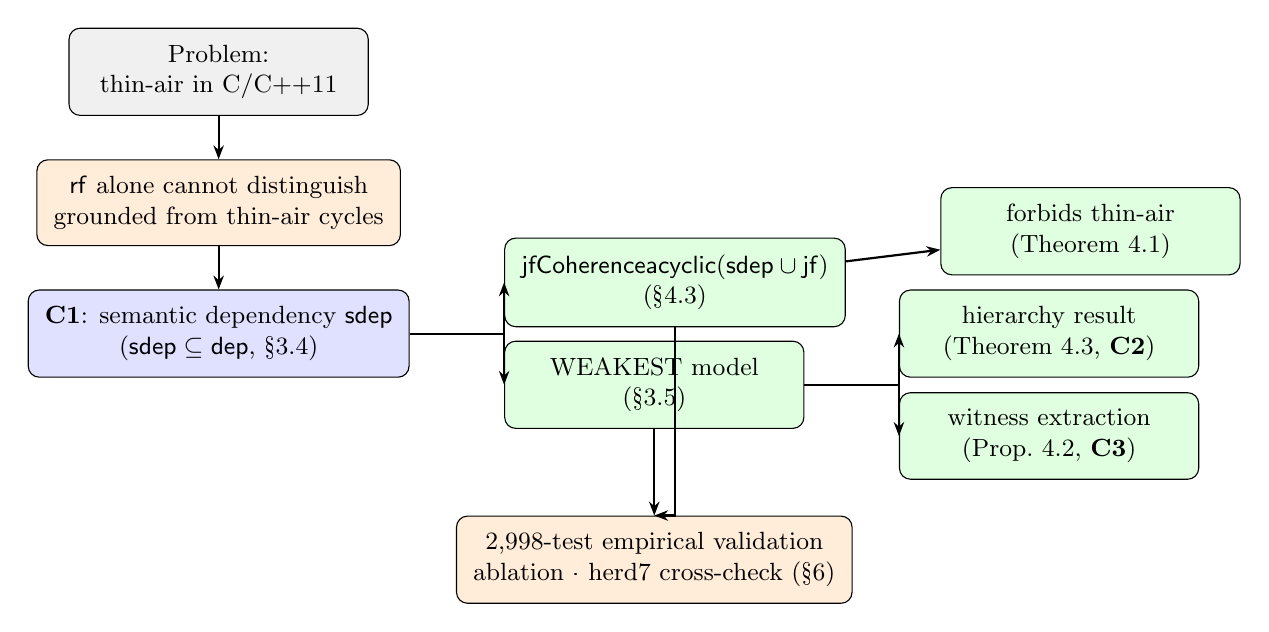
\begin{tikzpicture}[
  box/.style={draw, rounded corners=4pt, minimum width=3.8cm,
              minimum height=0.7cm, font=\small, inner sep=6pt,
              align=center},
  prob/.style={box, fill=gray!12},
  obs/.style={box, fill=orange!15},
  c1/.style={box, fill=blue!12},
  result/.style={box, fill=green!12},
  arr/.style={-{Stealth[length=5pt]}, thick},
  node distance=0.55cm and 1.2cm
]
 
%% Column 1 — Problem + Observation
\node[prob]  (prob)  {Problem:\\thin-air in C/C++11};
\node[obs, below=of prob] (obs)
  {$\rf$ alone cannot distinguish\\grounded from thin-air cycles};
\draw[arr] (prob) -- (obs);
 
%% Column 1 — C1
\node[c1, below=of obs] (c1)
  {\textbf{C1}: semantic dependency $\sdep$\\($\sdep \subseteq \dep$,\ §3.4)};
\draw[arr] (obs) -- (c1);
 
%% Branch right from C1: jfCoherence → soundness
\node[result, right=of c1, yshift=0.65cm] (jfc)
  {$\jfCoherence \triangleq \mathsf{acyclic}(\sdep \cup \jf)$\\(§4.3)};
\node[result, right=of jfc, yshift=0.65cm] (sound)
  {forbids thin-air\\(Theorem~4.1)};
\draw[arr] (c1.east) -| (jfc.west);
\draw[arr] (jfc) -- (sound);
 
%% Branch right-down from C1: WEAKEST model
\node[result, right=of c1, yshift=-0.65cm] (weak)
  {WEAKEST model\\(§3.5)};
\node[result, right=of weak, yshift=0.65cm] (hier)
  {hierarchy result\\(Theorem~4.3, \textbf{C2})};
\node[result, right=of weak, yshift=-0.65cm] (wit)
  {witness extraction\\(Prop.~4.2, \textbf{C3})};
\draw[arr] (c1.east) -| (weak.west);
\draw[arr] (weak.east) -| (hier.west);
\draw[arr] (weak.east) -| (wit.west);
 
%% Evaluation node below everything
\node[obs, below=1.1cm of weak] (eval)
  {2,998-test empirical validation\\ablation · herd7 cross-check (§6)};
\draw[arr] (jfc.south) |- (eval.north);
\draw[arr] (weak.south) -- (eval.north);
 
\end{tikzpicture}
\caption{Contribution map. The central observation (rf alone is insufficient) motivates
semantic dependency $\sdep$ (C1), from which $\jfCoherence$ and the WEAKEST model
follow. The hierarchy result (C2) and witness extraction (C3) build on the WEAKEST
encoding. All three contributions are corroborated by empirical validation on 2,998
supported-syntax litmus tests.}
\Description{A node and arrow diagram showing the contribution map.}
\label{fig:contrib-map}
\end{figure}

%%% §1 Introduction
\section{Introduction}
\label{sec:intro}

The C/C++11 thin-air problem~\cite{boehmDemsky2014outlawing,batty2015problem}
is a persistent gap in the semantics of relaxed atomics. The standard permits
implementations to compile \texttt{memory\_order\_relaxed} accesses to bare
loads and stores, exposing the load-buffering reorderings that current ARM and
Power hardware exhibit. But the same flexibility admits executions in which a
group of reads justifies one another cyclically, fabricating values with no
causal origin in the initial state or any prior write. The C++ standard itself
acknowledges this in a non-normative note (29.3p11) but provides no semantic
mechanism to forbid such executions; the LB+ctrldata+ctrl-single program of
Batty et al.\ is the paradigmatic case. Our checker forbids ctrl-single
correctly; it also conservatively forbids ctrl-double, the companion program
that must be allowed---a known limitation of the per-execution setting for
control dependencies, discussed in \S\ref{sec:limitations}.

The difficulty is not that thin-air executions are hard to recognize
informally. The difficulty is that every per-execution adaptation of the
C/C++11 candidate-execution discipline either over-forbids the load-buffering
executions that the language must allow~\cite{lahav2017repairing}, or admits
cyclic justifications without causal support. Batty et
al.~\cite[Theorem~2]{batty2015problem} make this precise: no adaptation of
the C/C++11 consistency predicate that uses the same notion of candidate
execution can give the desired behavior for both the program that must be
allowed (a vacuous conditional collapsing under compiler optimization) and the
program that must be forbidden (a self-satisfying conditional). The published
resolutions therefore leave the per-execution setting: Chakraborty and
Vafeiadis~\cite{chakraborty2019grounding} construct event structures with a
visibility predicate that quantifies over conflicting branches; Kang et
al.~\cite{kang2017promising} adopt an operational promise-and-certify
discipline that quantifies over thread-local continuations.

The obstacle in Batty et al.'s negative result can be named precisely: two
load-buffering programs of identical $\po \cup \rf$ shape can differ in whether
their data dependencies carry genuine value-flow---one thread writing $r$
(a copy of the read value, value-dependent) versus $r \oplus r \oplus 1$ (constant regardless of $r$).
The first is thin-air and must be forbidden; the second is grounded and must be
allowed. Distinguishing them is a \emph{value-flow} question on a single
execution, not a cross-branch reasoning question.

The structure we add is a semantic-dependency subrelation $\sdep \subseteq
\dep$, where $\dep$ is the standard data-address-control syntactic dependency
relation. A dependency $(p, c)$ is \emph{semantic} iff $c$'s computed value,
accessed location, or control outcome genuinely depends on the value read at
$p$. Equivalently, there exist two assignments of values to the program's
reads, agreeing on every read except $p$, under which $c$'s outcome differs.
Dependencies that fail this---the canonical
instance being a write of $r \oplus r$, whose value is independent of
$r$---are \emph{fake}. Our consistency condition for the WEAKEST model is
$\jfCoherence \triangleq \mathsf{acyclic}(\sdep \cup \jf)$, where $\jf$ is
the per-read justification primitive~\cite{chakraborty2019grounding}
coincident with $\rf$ on single executions. On the two load-buffering programs
above, the real data dependency is in $\sdep$, the cycle survives, and the
thin-air outcome is FORBIDDEN; the fake data dependency is in $\dep \setminus
\sdep$, no cycle exists, and the grounded outcome is ALLOWED. We have verified
this directly: our prototype returns the expected verdict on both, and confirms
that removing the semantic-dependency input from the encoder flips the thin-air
case to satisfiable.

Our position relative to the published resolutions is precise, and requires
answering three questions a reviewer will ask.

\paragraph{Why not RC11?}
RC11~\cite{lahav2017repairing} forbids all $\mathsf{sb} \cup \rf$ cycles,
blocking grounded LB along with thin-air. Relaxing $\mathsf{sb}$ without
value-flow information either re-admits thin-air or requires exactly $\sdep$.
Our checker uses $\mathsf{acyclic}(\sdep \cup \jf)$, admitting grounded LB
on data/address dependencies (\S\ref{sec:rc11baseline}).

\paragraph{Why not Promising?}
Promising~\cite{kang2017promising} certifies writes by exhibiting future
executions---structurally off-candidate. It cannot be a per-candidate predicate
by design (\S\ref{sec:related}).

\paragraph{Why not Weakestmo?}
Weakestmo~\cite{chakraborty2019grounding} defines grounding via event-structure
construction order---no per-candidate analogue exists. Restricting it to one
execution re-derives $\sdep$ (\S\ref{sec:semdep}).

\paragraph{Why not PwT?}
PwT~\cite{jeffrey2022leaky} has axiom $\mathsf{acyclic}(\rf \cup
\sdep_{\mathrm{PwT}})$ identical to $\jfCoherence$, but PwT's $\sdep$ is
multi-execution. Ours is per static site---decidable offline, SMT-encodable
(\S\ref{sec:related}).

\noindent All four approaches exit the per-execution setting or over-forbid. Our checker shows this setting is sufficient for data/address dependencies: $\sdep$ is answered once offline, and $\mathsf{acyclic}(\sdep \cup \jf)$ decides thin-air on a single candidate. Cost: conservatism on control dependencies (\S\ref{sec:limitations}).

\noindent\textbf{Conceptual contribution.}
We show that distinguishing semantic from syntactic dependencies is sufficient
to recover grounded load-buffering on data and address dependencies while excluding thin-air, within a single-execution consistency framework and without appeal to event-structure construction or operational certification.

\noindent The paper makes three technical contributions.
\textbf{C1 (\S\ref{sec:semdep}, \S\ref{sec:minimality}, \S\ref{sec:jfcoherence}).}
We introduce $\sdep$ as the additional structure beyond $\rf$ required to
distinguish grounded from thin-air cyclic justification on a single execution,
and show that $\sdep$ is the unique maximal adequate relation (on data and
address dependency edges; \S\ref{sec:minimality}) satisfying this
characterization (Proposition~\ref{prop:sdep-maximal}).
From this characterization we define $\jfCoherence \triangleq
\mathsf{acyclic}(\sdep \cup \jf)$ and show that the resulting
WEAKEST-consistency predicate is sound for forbidding thin-air on the
supported-syntax fragment (Theorem~\ref{thm:soundness}).
\textbf{C2 (\S\ref{sec:hierarchy}).}
We characterize the model lattice under our encoding: SC dominates each weak
model by construction (Theorem~\ref{thm:hierarchy}), and the intermediate
edges of the conventional chain do not hold under our axiom sets
(Propositions~\ref{prop:tso-pso} and~\ref{prop:ra-weakest}). These are
facts about our specific encoding (noted in \S\ref{sec:hierarchy}); the
PSO encoding diverges from canonical SPARC PSO and the result should be read
as encoder validation rather than a claim about standard weak memory models.
\textbf{C3 (\S\ref{sec:witness}).}
We give a minimum-cardinality witness extraction procedure that, for a model
$M$ and a target predicate, returns either an execution of minimum
active-event cardinality consistent under $M$ and satisfying the predicate,
certified by an optimizer's OPT status, or proof that none exists within a
stated budget (Proposition~\ref{thm:minwitness}).

\begin{table}[ht]
\centering
\caption{Design-space comparison. The three prior approaches each solve the
thin-air problem but exit the per-execution setting to do so. Our checker
identifies a per-execution realization of the same distinction.}
\label{tab:design-space}
\small
\begin{tabular}{llll}
\toprule
Approach & Representation & Thin-air mechanism & Fake-dep.\ distinction? \\
\midrule
RC11~\cite{lahav2017repairing}
  & candidate execution
  & $\mathsf{sb} \cup \rf$ acyclic
  & No (over-forbids LB) \\
Promising~\cite{kang2017promising}
  & operational (threads)
  & certification of future exec.
  & Yes (operationally) \\
Weakestmo~\cite{chakraborty2019grounding}
  & event structure
  & visibility predicate
  & Yes (multi-execution) \\
\textbf{This work}
  & \textbf{single candidate exec.}
  & $\mathsf{acyclic}(\sdep \cup \jf)$
  & \textbf{Yes (value-aware, per-exec.)} \\
\bottomrule
\end{tabular}
\end{table}

We validate the contributions on a 2,998-test supported-syntax fragment of a
12,324-file corpus drawn from the herd7 and Dat3M suites. A
three-configuration ablation (\S\ref{sec:ablation}) confirms that $\sdep$ is
empirically indispensable on the load-buffering family: removing it admits
thin-air, retaining it without stratification rejects grounded executions, and
the shipped detector is the only configuration that produces the correct verdict
on every member of that family. A
herd7 cross-check (\S\ref{sec:herd7}) on the shared strong-fragment subset
establishes that our checker's strong-mode disagreements are documented
under-approximations rather than soundness failures. A categorization of the
parser-failure complement (\S\ref{sec:coverage}) scopes the empirical claims
honestly to the supported-syntax fragment.

Existing per-execution approaches to thin-air occupy two extreme points in
the design space: preserve syntactic dependencies wholesale (as hardware
models and IMM do), rejecting compiler optimizations that erase them; or
reject cyclic justification entirely (as RC11 does), blocking grounded
load-buffering in the process. This work identifies a middle point: a
value-aware stratification of these dependencies into semantic and fake
that is sufficient---on the supported-syntax fragment---to admit grounded
load-buffering while forbidding Boehm-Demsky thin-air cycles
(Theorem~\ref{thm:soundness}), decided on a single candidate execution without
multi-execution machinery. The cost is the conservatism of the detector on
control dependencies; the benefit is decidability and the per-execution
discipline.

\paragraph{What this paper does not claim.}
We do not prove DRF, compositionality, or compilation correctness for the WEAKEST model; these require lifting the per-execution predicate to a multi-execution semantics (\S\ref{sec:limitations}). We do not prove a formal correspondence to Weakestmo or Promising. Mechanization is future work.

\S\S\ref{sec:background}--\ref{sec:programs} give background and definitions;
\S\ref{sec:consistency} develops the model and theorems; \S\ref{sec:detector}
describes $\sdepimpl$; \S\ref{sec:evaluation} reports the evaluation;
\S\ref{sec:related} positions the work; \S\ref{sec:limitations} states
limitations.


%%% §2 Background
\section{Background}
\label{sec:background}

Modern multiprocessors do not execute memory operations in program order.
Stores may be buffered, loads may be satisfied from local caches, and
independent operations may be reordered by the hardware or compiler. Weak
memory models formalise which reorderings are permitted by assigning meaning
to concurrent programs not via a single interleaved execution but via a set of
\emph{candidate executions}, each recording the events a thread performs and
the memory relations---reads-from ($\rf$), coherence ($\co$), from-reads
($\fr$)---that hold among
them~\cite{boehmAdve2008foundations,batty2015problem}. A program outcome is
permitted if some candidate execution satisfying the model's consistency axioms
witnesses it.

The \emph{thin-air problem}~\cite{boehmDemsky2014outlawing} is the canonical
deficiency of the C/C++11 relaxed-atomics fragment: per-execution axioms admit
cyclic justification where a value appears to cause itself. All published
resolutions exit the per-execution setting---via event structures
(Weakestmo~\cite{chakraborty2019grounding}), operational certification
(Promising~\cite{kang2017promising}), or by forbidding all load-buffering
(RC11~\cite{lahav2017repairing}). This paper asks whether the per-execution
setting can be retained.


%%% §3 The WEAKEST Model and its SMT Encoding
\section{The WEAKEST Model and its SMT Encoding}
\label{sec:programs}

\subsection{Programs}
\label{sec:programs-def}

A \emph{program} is a finite set of threads $T = \{t_1, \ldots, t_n\}$. Each
thread $t_i$ is a finite sequence of \emph{instructions}: reads
$r \leftarrow \mathtt{load}(x)$, writes $\mathtt{store}(x, e)$,
read-modify-write operations $r \leftarrow \mathtt{RMW}(x, e)$, and
control-flow instructions (conditionals and loops). Expressions $e$ are
integer-valued, formed from integer constants, thread-local registers, and the
arithmetic and bitwise operators of the C/C++11 relaxed fragment. Memory
locations $x \in \mathcal{X}$ are shared and word-sized; registers are
thread-local. The conceptual development of \S\ref{sec:consistency} is
independent of the current parser's supported-syntax fragment; the
supported-syntax fragment itself is described in \S\ref{sec:coverage}.

\subsection{Events and candidate executions}
\label{sec:executions}

Executing a program produces \emph{events}: a read event $R(x, v)$ records a
load of value $v$ from location $x$; a write event $W(x, v)$ records a store
of value $v$ to $x$; an RMW event $\mathit{RMW}(x, v_r, v_w)$ records an
atomic read of $v_r$ paired with a write of $v_w$ at $x$. A \emph{candidate
execution} $\mathcal{X} = (E, \po, \rf, \co)$ consists of a finite set of
events $E$, a \emph{program order} $\po \subseteq E \times E$ that totally
orders the events of each thread, a \emph{reads-from} relation $\rf \subseteq
W \times R$ that maps each read to a unique write of the same location and
value, and a \emph{coherence order} $\co$ that totally orders the writes to
each location. The \emph{from-reads} relation $\fr = \rf^{-1} \,;\, \co$ is
derived. A program's \emph{behavior} is the set of outcomes realizable in some
consistent candidate execution (\S\ref{sec:consistency}).

\subsection{Syntactic dependencies}
\label{sec:syndep}

The \emph{syntactic dependency} relation $\dep \subseteq R \times (R \cup W)$
is the standard data-address-control dependency relation over events. A
read-to-write \emph{data dependency} $(p, c) \in \dep_{\mathrm{data}}$ holds
when the value read at $p$ flows into the expression computing the value
written at $c$. A read-to-access \emph{address dependency} $(p, c) \in
\dep_{\mathrm{addr}}$ holds when the value read at $p$ flows into the
expression computing the address of $c$. A read-to-access \emph{control
dependency} $(p, c) \in \dep_{\mathrm{ctrl}}$ holds when the value read at $p$
influences, via a conditional or loop, whether $c$ executes. We set $\dep \triangleq \dep_{\mathrm{data}} \cup \dep_{\mathrm{addr}} \cup
\dep_{\mathrm{ctrl}}$. Every $\dep$ edge is syntactically observable from the
program text. By definition, for every $(p, c) \in \dep$, $p$ precedes $c$ in
the same thread's program order: $\dep \subseteq \po$. (Dependencies flow
forward along a single thread's instruction sequence; the target $c$ always
executes after the source read $p$.) This containment is used explicitly in
Theorem~\ref{thm:hierarchy}. The central question of this paper is which of
these syntactic dependencies carry genuine value-flow and therefore participate
in cyclic justification; that question is taken up in \S\ref{sec:semdep}.

\subsection{Semantic dependence}
\label{sec:semdep}

Not every syntactic dependency carries genuine value-flow. We single out the
\emph{semantic dependencies}
\[
  \sdep \subseteq \dep,
\]
where $(p, c) \in \sdep$ iff $c$ genuinely depends on the value observed at
$p$: there exist two assignments of values to the program's read events,
agreeing on the value at every read except $p$, such that either (i)~$c$
executes under both assignments and $c$'s \emph{outcome} differs between them,
or (ii)~$c$ executes under exactly one of the two assignments (execution-sensitivity).
Here, outcome for case~(i) means: the value written (for a write event $c \in
W$) or the address accessed (for an address-dependent $c$). Case~(ii) covers
control-dependent events: if varying $p$'s value changes whether $c$ executes
at all, the dependency is semantic regardless of $c$'s label. Reads are treated as
unconstrained inputs---their values are not required to be rf-justified by any
execution. A dependency in $\dep \setminus \sdep$ is \emph{fake}---syntactically
present but semantically vacuous, the canonical instance being a write of
$r \oplus r$, whose value is independent of $r$.

The free-valuation formulation avoids circularity ($\sdep$ cannot be defined via executions of a model that uses $\sdep$) and is faithful to what the definition asks: expression-level value-dependence is a property of the expression alone, independent of how values arise in any execution.

Event-structure models in the Weakestmo
tradition~\cite{chakraborty2019grounding} do not stratify dependencies:
thin-air is addressed structurally, via a visibility predicate over the
incremental construction of event structures, which blocks reads whose
justifications recursively depend on conflicting writes lacking equal-write
replacements in the read's own branch. In the single-execution setting we
cannot appeal to construction-time visibility, and we instead introduce $\sdep$
as a primitive value-sensitive relation; \S\ref{sec:jfcoherence}'s
$\jfCoherence$ axiom is stated purely over $\sdep$.

$\sdep$ is a static property of a dependency \emph{site} $(p,c)$ in the
program text---it asks whether the write expression at $c$ changes when the
value at source read $p$ changes, treating all read values as independent
inputs. Formally, $\sdep$ is decided per static site and then lifted to
events: an event-level edge $(p, c) \in \dep$ of a candidate execution is in
(event-level) $\sdep$ iff the static site it instantiates is semantic. All
uses of $\sdep$ over executions (in particular \jfCoherence) refer to this
lifting; site-uniformity, used in Proposition~\ref{prop:sdep-maximal}, is
automatic for $\sdep$ by construction. The question is answered once per
static dependency edge, prior to and
independent of consistency-checking any particular candidate execution.
Consistency-checking a candidate execution $\mathcal{X}$ then consumes the
resulting (already-computed) $\sdep$ relation as a fixed input and performs a
single per-execution acyclicity check, $\mathsf{acyclic}(\sdep \cup \jf)$,
over $\mathcal{X}$ alone.

This locates $\sdep$ precisely: it is decidable exactly when program-level
equivalence of the relevant sub-expressions is decidable, which for the
arithmetic and bitwise fragment of \S\ref{sec:programs-def} is a bounded
symbolic-equivalence problem, not an open one.

\S\ref{sec:detector} gives the conservative syntactic approximation
$\sdepimpl$ our prototype computes, satisfying $\sdeptrue \subseteq \sdepimpl
\subseteq \dep$ (Lemma~\ref{lem:detector-soundness}); it inherits $\sdep$'s
per-site, per-program character rather than approximating anything
execution-specific. Two implementation choices, justified in
\S\ref{sec:detector}, affect the $\sdepimpl$ used throughout: address
dependencies are subject to the same syntactic approximation as data
dependencies, while \textbf{control dependencies are conservatively retained
as semantic}---$\dep_{\mathrm{ctrl}} \subseteq \sdepimpl$---since
control-dependency cancellation under weak memory is architecture-sensitive
and our prototype does not attempt it. This conservative inclusion means
$\sdepimpl$ may strictly over-approximate $\sdeptrue$ on control
dependencies; the over-approximation is safe (Theorem~\ref{thm:soundness})
but may forbid a small class of grounded executions whose control structure
encodes a fake dependency. We have not encountered such an execution in the
corpus (the LB-real/LB-fake matched pair of \S\ref{sec:matched-pair} is the
canonical instance where this distinction does and does not fire).

\subsection{The WEAKEST consistency predicate}
\label{sec:weakest}

A candidate execution $\mathcal{X}$ is \emph{WEAKEST-consistent} if it
satisfies three axioms.

\textbf{CoherencePerLocation:} $\mathsf{acyclic}(\po_{\mathrm{loc}} \allowbreak \cup \rf \allowbreak \cup \co \allowbreak \cup \fr)$, where $\po_{\mathrm{loc}}$ restricts $\po$ to pairs of
events at the same location. This is the standard per-location coherence
requirement shared by all five encoded models.

\textbf{RMWAtomicity:} for every RMW event the read-part and write-part are
adjacent in $\co$: no write $w'$ satisfies both $\co(w_{\mathit{pre}}, w')$ and $\co(w',
w)$, where $w$ is the write-half and $w_{\mathit{pre}}$ is the write that the
RMW's read-half reads from (i.e., $(w_{\mathit{pre}}, r) \in \rf$ where $r$
is the read-half). This ensures atomicity of read-modify-write operations
and is shared across all five models.

\textbf{jfCoherence:} $\mathsf{acyclic}(\sdep \cup \jf)$, as defined in
\S\ref{sec:jfcoherence}. In the prototype the abstract relation $\sdep$ is
replaced by its conservative approximation $\sdepimpl$ (\S\ref{sec:detector});
the abstract formulation is stated over $\sdep$. The first two axioms are
shared with SC, TSO, PSO, and RA; jfCoherence is the WEAKEST-specific axiom
that distinguishes semantic from syntactic dependencies and rules out thin-air.

\subsection{SMT encoding}
\label{sec:smt}

Each consistency predicate is encoded as a quantifier-free first-order formula
over the events of a candidate execution. Events are represented as
integer-indexed constants; binary relations are encoded as Boolean matrices.
Acyclicity of a relation $R$ is encoded by the existence of a strict total
order (topological sort) $\prec$ on the events such that $(e, e') \in R
\Rightarrow e \prec e'$~\cite{gavrilenko2019bmc}; this introduces $O(|E|^2)$
Boolean variables and $O(|E|^2)$ clauses. Reads-from is encoded directly from
the candidate wiring produced by the loader. Coherence order $\co$ is encoded
as a decision variable subject to the total-order and CoherencePerLocation
constraints. The resulting formula is discharged by Z3; satisfiability
witnesses a consistent candidate, unsatisfiability refutes it. The five models
(SC, TSO, PSO, RA, WEAKEST) differ only in which acyclicity constraints are asserted, making the encoding modular: the WEAKEST encoding adds the $\sdepimpl$ matrix and the $\jfCoherence$ acyclicity constraint to the shared
CoherencePerLocation and RMWAtomicity base.


%%% §4 Semantic vs. Syntactic Dependencies
\section{Semantic vs.\ Syntactic Dependencies}
\label{sec:consistency}

\subsection{Scope}
\label{sec:scope}

We work in the per-candidate-execution setting of axiomatic memory models. A
candidate execution is a tuple of events, a program order $\po$, a reads-from
relation $\rf$, a coherence order $\co$, and the derived from-read relation
$\fr = \rf^{-1} ; \co$. A consistency predicate is a boolean function over
candidate executions; a program's behavior is the set of values realizable in
some consistent candidate. This is the discipline of
C/C++11~\cite{batty2015problem}, RC11~\cite{lahav2017repairing},
IMM~\cite{podkopaev2019bridging}, and many others. It is decidable on a single
candidate (the candidate is finite, the predicate is first-order over its
relations), which is the property we exploit.

We operate in this setting on the WEAKEST model defined in
\S\ref{sec:weakest}; the four standard models (SC, TSO, PSO, RA) are encoded
for comparison and for the hierarchy theorem of \S\ref{sec:hierarchy}. The
reasons Weakestmo and Promising cannot be reduced to the per-candidate setting
are given in \S\ref{sec:intro} and \S\ref{sec:related}; this section develops
that formalism directly.

We encode the predicate in SMT. The encoder produces a quantifier-free
first-order constraint over the events of a candidate execution; the SMT
solver Z3~\cite{demoura2008z3} discharges satisfiability or returns a model.
Acyclicity constraints over binary relations are encoded via a topological-sort
witness function~\cite{gavrilenko2019bmc}. Minimum-cardinality witness
extraction (\S\ref{sec:witness}) uses Z3's Optimization Modulo Theory
mode~\cite{bjorner2015nuz}.

\subsection{The matched pair: LB-real and LB-fake}
\label{sec:matched-pair}

\begin{figure}[t]
\centering
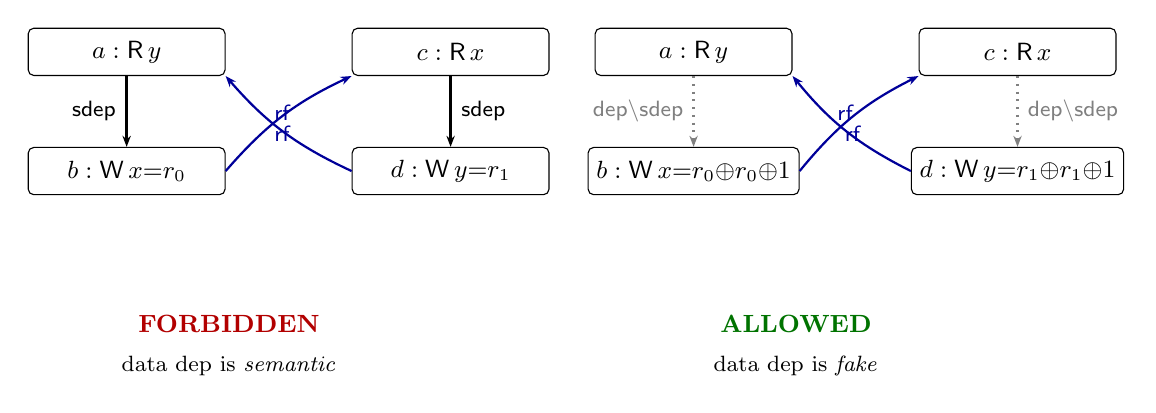
\begin{tikzpicture}[
  ev/.style={draw, rounded corners=2pt, minimum width=2.5cm,
             minimum height=0.6cm, font=\small, inner sep=3pt, align=center},
  rfedge/.style={-{Stealth[length=4pt]}, thick, color=blue!60!black},
  sdepedge/.style={-{Stealth[length=4pt]}, very thick},
  fakeedge/.style={-{Stealth[length=4pt]}, thick, dotted, color=gray},
  lbl/.style={font=\footnotesize},
  node distance=0.9cm and 0.6cm
]

%% ===== LEFT: LB-real =====
\node[ev] (a1) {$a:\mathsf{R}\,y$};
\node[ev, below=of a1] (b1) {$b:\mathsf{W}\,x{=}r_0$};
\node[ev, right=1.6cm of a1] (c1) {$c:\mathsf{R}\,x$};
\node[ev, below=of c1] (d1) {$d:\mathsf{W}\,y{=}r_1$};

\draw[sdepedge] (a1) -- node[lbl,left]{$\sdep$} (b1);
\draw[sdepedge] (c1) -- node[lbl,right]{$\sdep$} (d1);
\draw[rfedge] (b1.east) to[bend left=12] node[lbl,below]{$\rf$} (c1.south west);
\draw[rfedge] (d1.west) to[bend left=12] node[lbl,above]{$\rf$} (a1.south east);

\node[font=\small\bfseries, below=1.4cm of b1, xshift=1.3cm] (v1)
  {\textcolor{red!70!black}{FORBIDDEN}};
\node[lbl, below=0.05cm of v1] {data dep is \emph{semantic}};

%% ===== RIGHT: LB-fake =====
\begin{scope}[xshift=7.2cm]
\node[ev] (a2) {$a:\mathsf{R}\,y$};
\node[ev, below=of a2] (b2) {$b:\mathsf{W}\,x{=}r_0{\oplus}r_0{\oplus}1$};
\node[ev, right=1.6cm of a2] (c2) {$c:\mathsf{R}\,x$};
\node[ev, below=of c2] (d2) {$d:\mathsf{W}\,y{=}r_1{\oplus}r_1{\oplus}1$};

\draw[fakeedge] (a2) -- node[lbl,left]{$\dep{\setminus}\sdep$} (b2);
\draw[fakeedge] (c2) -- node[lbl,right]{$\dep{\setminus}\sdep$} (d2);
\draw[rfedge] (b2.east) to[bend left=12] node[lbl,below]{$\rf$} (c2.south west);
\draw[rfedge] (d2.west) to[bend left=12] node[lbl,above]{$\rf$} (a2.south east);

\node[font=\small\bfseries, below=1.4cm of b2, xshift=1.3cm] (v2)
  {\textcolor{green!45!black}{ALLOWED}};
\node[lbl, below=0.05cm of v2] {data dep is \emph{fake}};
\end{scope}

\end{tikzpicture}

\fbox{\begin{minipage}{0.9\linewidth}
\centering\small
Same $\po$. \quad Same $\rf$. \quad Same observed values
($r_0{=}r_1{=}1$). \quad \textbf{Different required verdicts.}\\
\textbf{$\rf$ alone cannot distinguish them; $\sdep$ can.}
\end{minipage}}

\caption{The matched pair. Both candidates wire the identical
$\po \cup \rf$ graph and realize the same values. They differ only in whether
the read-to-write data dependency is semantic. In LB-real, the copy $r$ depends on
$r$, so the edge enters $\sdep$ and $\jfCoherence$ closes the cycle
(FORBIDDEN). In LB-fake, $r \oplus r \oplus 1$ is constant in $r$, so the edge
lies in $\dep \setminus \sdep$, no cycle exists, and the grounded outcome is
admitted (ALLOWED).}
\Description{Two side-by-side node diagrams showing the identical structure of LB-real and LB-fake but with semantic and fake dependencies.}
\label{fig:matched-pair}
\end{figure}

The matched pair is the central exhibit of this paper. We present two
load-buffering programs with \emph{identical} $\po \cup \rf$ structure and
\emph{identical} observed values, but \emph{different} required verdicts.
Their difference isolates exactly the information that observational
reads-from cannot provide. In both programs the shared locations $x$ and $y$
are initialised to~0, so any candidate in which a read observes~1 must take
that value from a thread write; the value~1 has no origin in the initial
state.

\paragraph{LB-real.}
Thread~1 reads $y$, writes $x = r_0$ (a copy). Thread~2 reads $x$, writes
$y = r_1$ (a copy). Consider the candidate execution in which both reads
observe value~1: $r_0 = r_1 = 1$, each thread writes~1 (copying what it
read), and the cyclic wiring has each thread reading from the other's write
of value~1. This wiring is value-consistent: each read observes~1 from a
write of~1. The written value $r$ genuinely depends on the value read: if
$r = 0$ the write is~0; if $r = 1$ the write is~1. The data dependency is
\emph{semantic}---it enters $\sdep$. The candidate contains a cycle in
$\sdep \cup \jf$. \jfCoherence{} forbids it. \textbf{Verdict: FORBIDDEN.}

\paragraph{LB-fake.}
Thread~1 reads $y$, writes $x = r_0 \oplus r_0 \oplus 1$. Thread~2
reads $x$, writes $y = r_1 \oplus r_1 \oplus 1$. The expression
$r \oplus r \oplus 1$ evaluates to~1 regardless of~$r$: it is a
constant. The $\po \cup \rf$ graph is identical to LB-real. The
observed values are identical. But the written value does not depend
on the value read. The data dependency is \emph{fake}---it lies in
$\dep \setminus \sdep$. No cycle exists in $\sdep \cup \jf$.
\jfCoherence{} admits it. \textbf{Verdict: ALLOWED.}

\paragraph{What the pair establishes.}
The two candidates agree on every observable: same program-order edges,
same reads-from edges, same values at every memory location. Any
consistency criterion based solely on observational $\rf$ must assign
them the same verdict. Since the required verdicts differ, no
$\rf$-only criterion is adequate. Semantic dependency is not a
convenience; it is \emph{the missing information} that a per-execution
criterion requires. This is the content of~C1. Figure~\ref{fig:matched-pair}
shows the two candidates side by side.

\begin{center}
\fbox{\begin{minipage}{0.88\linewidth}
\textbf{Takeaway.}
Same $\po$.
Same $\rf$.
Same observed values.
Different required verdicts.
Therefore no consistency criterion using only observational $\rf$ is
adequate to distinguish grounded from thin-air cyclic justification.
$\sdep$ is the missing information. This is C1.
\end{minipage}}
\end{center}

\subsection{Justifying the choice of $\sdep$}
\label{sec:minimality}

The matched pair of \S\ref{sec:matched-pair} establishes that $\rf$ alone is
insufficient. We now show $\sdep$ is the strongest relation that can be added
while remaining sound. A binary relation $R \subseteq E \times E$ is
\emph{adequate} if it is \emph{site-uniform} (membership determined by the
static dependency site, identically across programs) and satisfies:
\begin{itemize}
  \item[(A1)] \textbf{Soundness.} For every program $P$ in the supported-syntax
    fragment and every candidate execution $\mathcal{X}$ of $P$: if
    $\mathsf{acyclic}(R \cup \jf)$ holds on $\mathcal{X}$, then $\mathcal{X}$
    does not contain a Boehm-Demsky thin-air cycle.
  \item[(A2)] \textbf{Grounded LB admission.} Every candidate execution of a
    two-thread load-buffering program in the supported-syntax fragment in which
    both writes produce a constant value (independent of what was read) is
    $\mathsf{acyclic}(R \cup \jf)$-consistent. (The LB-fake candidate of
    \S\ref{sec:matched-pair} is the canonical instance.)
  \item[(A3)] \textbf{LB-real rejection.} The candidate execution of LB-real
    (\S\ref{sec:matched-pair}) is not $\mathsf{acyclic}(R \cup \jf)$-consistent.
\end{itemize}



\begin{proposition}[Maximality of $\sdep$ among adequate relations]
\label{prop:sdep-maximal}
$\sdep$ is the \emph{largest} (by set inclusion) adequate relation on
data and address dependency edges: for any adequate relation $R$ restricted to
$\dep_{\mathrm{data}} \cup \dep_{\mathrm{addr}}$, we have $R \subseteq \sdep$.
\end{proposition}

The proof uses the following construction lemma.

\begin{lemma}[LB embedding of fake data/address edges]
\label{lem:lb-embedding}
Let $e = (p, c) \in (\dep_{\mathrm{data}} \cup \dep_{\mathrm{addr}}) \setminus
\sdep$ be any fake data or address dependency edge in the supported-syntax
fragment. Then there exists a two-thread load-buffering program $P_e$ in the
supported-syntax fragment and a candidate execution $\mathcal{X}_e$ of $P_e$
such that: (i) $e$'s dependency role appears in $P_e$'s read-to-write path;
(ii) $e \notin \sdep(P_e)$ (the edge is fake in $P_e$ as well, since
value-independence is preserved by embedding); and (iii) $\mathcal{X}_e$
is grounded---both writes produce a constant $k$ independent of the values
read---so the required verdict for $\mathcal{X}_e$ is ALLOWED.
\end{lemma}
\begin{proof}[Proof of Lemma~\ref{lem:lb-embedding}]
Since $e \notin \sdep$, the write expression at $c$ evaluates to a value $k$
independent of the value read at $p$ (\S\ref{sec:semdep}). Construct $P_e$
as follows. Thread~1 reads location $y$ (producing event $p$), then writes
$x$ using the same expression as $c$---which evaluates to $k$ regardless of
the value read at $p$---yielding event $c$ with value $k$. Thread~2 mirrors:
reads $x$ (producing event $p'$), writes $y$ using the same expression,
yielding event $c'$ with value $k$. For a fake \emph{address} dependency,
the same construction applies with $c$'s expression computing the target
address rather than the written value: the address evaluates to a fixed
location $\ell$ regardless of the value read at $p$, so the wiring is grounded
in the same sense. The programs are in the supported-syntax
fragment because $c$'s expression is already in the supported fragment (it is
a sub-expression of an event in the original program). The candidate
$\mathcal{X}_e$ wires $p$ to read from $c'$ and $p'$ to read from $c$, both
observing value $k$. Since both writes produce $k$ unconditionally, this wiring is grounded.
$\mathcal{X}_e$ is a valid candidate execution of $P_e$: $\po$ totally orders
each thread's two events; $\rf$ maps each read to a write of the same location
and value ($k$); $\co$ orders the two writes to each location; $\fr$ is
derived. $\mathcal{X}_e$ satisfies \textsf{CoherencePerLocation} (no location
has a coherence cycle) and \textsf{RMWAtomicity} vacuously (no RMW events).
The $\po \cup \rf$ graph of $\mathcal{X}_e$ is the standard LB shape, and
$e \notin \sdep(P_e)$ because $\sdep$-membership is defined by the
free-valuation criterion on the expression at $c$ (\S\ref{sec:semdep}):
$(p,c) \in \sdep$ iff two assignments of values to the program's reads, agreeing
on every read except $p$, produce different outcomes at $c$. Since $c$'s expression in $P_e$ is
identical to its expression in the original program, and value-independence (the
expression evaluates to the same constant $k$ regardless of $p$'s value) is a
property of that expression alone, $e \notin \sdep(P_e)$ follows directly from
$e \notin \sdep$ in the original program.
\end{proof}

\par\noindent\textbf{Scope of this result.}
\begin{description}[nosep,style=nextline,leftmargin=6.5em,labelwidth=6em]
  \item[\textit{Assumed:}] $\sdep$ is defined by the free-valuation criterion of \S\ref{sec:semdep}; $c$'s expression is in the supported-syntax fragment.
  \item[\textit{Proved:}] For every fake data/address edge $e$, an LB program $P_e$ exists (in the supported-syntax fragment) such that $e$ plays the fake-dependency role and the required verdict is ALLOWED.
  \item[\textit{Not proved:}] That $P_e$ is unique; that the construction extends to control dependencies (it does not).
\end{description}
\par
\begin{proof}[Proof of Proposition~\ref{prop:sdep-maximal}]
Let $R$ be adequate. We show $R \subseteq \sdep$ on data and address edges.
Take any fake edge $e = (p, c) \in (\dep_{\mathrm{data}} \cup
\dep_{\mathrm{addr}}) \setminus \sdep$; we show $e \notin R$.

By Lemma~\ref{lem:lb-embedding}, there exists a grounded LB program $P_e$
with candidate $\mathcal{X}_e$ in which $e$'s expression plays the fake
data-dependency role and the required verdict is ALLOWED. By Lemma~\ref{lem:lb-embedding}, $\mathcal{X}_e$ is grounded (both writes
produce $k$ unconditionally). Condition~(A2) therefore directly requires
$\mathsf{acyclic}(R \cup \jf)$ on $\mathcal{X}_e$.

The $\jf$ edges of $\mathcal{X}_e$ form the standard LB cyclic wiring. For
$\mathsf{acyclic}(R \cup \jf)$ to hold despite this cyclic $\jf$, the
$R$-edge along the dependency path must not close the cycle. The LB program
$P_e$ has two dependency edges, one per thread, both instantiating the same
static site $e$; site-uniformity of $R$ ensures both are in $R$ or both are
absent. For acyclicity to hold, both must be absent---which requires $e \notin R$.
Since $e$ was arbitrary in $\dep_{\mathrm{data}} \cup
\dep_{\mathrm{addr}} \setminus \sdep$, we have $R \subseteq \sdep$ on these
edges.

(A1) follows from the containment argument of Theorem~\ref{thm:soundness} with $\sdeptrue = \sdep$; (A2) holds because fake edges are outside $\sdep$ by definition, so no cycle closes on grounded LB; (A3) holds because the genuine dependency of LB-real is in $\sdep$ by definition.
\end{proof}

\par\noindent\textbf{Scope of this result.}
\begin{description}[nosep,style=nextline,leftmargin=6.5em,labelwidth=6em]
  \item[\textit{Assumed:}] Site-uniformity and adequacy conditions (A1)--(A3) as defined above; Lemma~\ref{lem:lb-embedding}.
  \item[\textit{Proved:}] Within the class of site-uniform adequate relations of the form $\mathsf{acyclic}(R \cup \jf)$, $\sdep$ is the unique maximal element under set inclusion on data and address dependency edges.
  \item[\textit{Not proved:}] Maximality over non-site-uniform adequate relations; maximality on control dependency edges.
\end{description}
\par

Two qualifications are necessary. First, this result is scoped to relations
of the form $\mathsf{acyclic}(R \cup \jf)$; it says nothing about consistency
criteria of a different syntactic form (e.g., criteria that use additional
per-read justification structure rather than a single binary relation). Second,
control dependencies fall outside Proposition~\ref{prop:sdep-maximal}: the
argument for fake-edge exclusion uses an LB-like construction, but
fake control-dependency detection requires cross-branch equivalence reasoning
(Batty et al.~\cite{batty2015problem}, \S\ref{sec:related}), which is
unavailable per-execution. The proposition is therefore strongest for data
and address dependencies, where $\sdep$ is provably maximal, and weaker (but
still sound) for control, where we conservatively include all edges.

\subsection{jfCoherence: the value-aware consistency condition}
\label{sec:jfcoherence}

We now define the consistency condition at the heart of the WEAKEST model:
\[
  \jfCoherence \;\triangleq\; \mathsf{acyclic}(\sdep \cup \jf).
\]
Read this directly: an execution is jf-coherent exactly when the union of the
semantic-dependency relation $\sdep$ and the justified-from relation $\jf$
contains no cycle. The relation $\jf$ records, for each read, the write it
takes its value from; on a single candidate execution it coincides with $\rf$. We retain the $\jf$ name for terminological continuity with Weakestmo~\cite{chakraborty2019grounding}, which defines justified-from over event structures where it diverges from $\rf$; on a single execution, one may read $\jf$ as $\rf$ throughout.
A thin-air cycle is a cycle of reads each justifying the next through a
\emph{genuine} value dependency---and a genuine value dependency is, by
definition (\S\ref{sec:semdep}), an $\sdep$ edge. The jfCoherence axiom forbids
exactly these cycles: it closes a cycle when the dependencies carrying it are
semantic, and leaves the graph acyclic when they are fake. This is why the
axiom admits LB-fake and forbids LB-real on the identical $\po \cup \rf$ graph
of \S\ref{sec:matched-pair}: the two candidates differ only in whether the
read-to-write edge enters $\sdep$, and that single difference is what
$\mathsf{acyclic}(\sdep \cup \jf)$ tests.

A note on the admission direction: when we say jfCoherence ``admits grounded
load-buffering,'' this is a claim about the per-site syntactic definition of
$\sdep$---executions whose write expressions are value-independent under the
free-valuation criterion of \S\ref{sec:semdep} are outside the cycle. It is
not a claim about compiler-reachable behaviours: a compiler with a range
invariant could eliminate a dependency our criterion classifies as semantic,
yielding a behaviour the compiled program exhibits but that jfCoherence would
forbid. Compilation correctness requires lifting to a multi-execution semantics
and is out of scope (\S\ref{sec:limitations}).

\subsection{Soundness of \texorpdfstring{$\jfCoherence$}{jfCoherence} on the supported-syntax fragment}
\label{sec:soundness}

Boehm and Demsky's articulation of thin-air is deliberately informal; to make
Theorem~\ref{thm:soundness} checkable we first fix a formal rendering of it in
our vocabulary, and we state explicitly that the theorem's soundness is
relative to this rendering.

\begin{definition}[Thin-air cycle]
\label{def:thin-air}
A candidate execution $\mathcal{X}$ exhibits a \emph{thin-air cycle} if there
exist reads $r_1, \ldots, r_n$ and writes $w_1, \ldots, w_n$ in $\mathcal{X}$
such that each $r_i$ takes its value from $w_i$ (i.e., $(w_i, r_i) \in \jf$)
and each write's value genuinely depends on the preceding read---formally,
$(r_{i-1}, w_i) \in \sdeptrue$, indices modulo $n$. This formalises the
Boehm--Demsky notion~\cite{boehmDemsky2014outlawing} of a value ``supported
only by self-justifying reads'': genuine value dependence is exactly
membership in $\sdeptrue$ (\S\ref{sec:semdep}), so fake dependencies
(e.g.\ $r \oplus r$) cannot carry a thin-air cycle, matching Boehm and
Demsky's own treatment of cancellation idioms.
\end{definition}

\paragraph{Fidelity of Definition~\ref{def:thin-air}.}
Definition~\ref{def:thin-air} is not a new proposal for what thin-air
means. It is a formal rendering of the Boehm--Demsky intuition---a value
``supported only by self-justifying reads''---in the vocabulary of
$\sdeptrue$ and $\jf$ that makes Theorem~\ref{thm:soundness} checkable.
The rendering is a choice, not a discovery; we make it explicit so the
theorem's scope is unambiguous. Table~\ref{tab:fidelity} verifies that this
rendering agrees with the literature's own classifications on every published
canonical example, including programs from Boehm--Demsky, Batty et al.,
Kang et al.\ (Promising), Jeffrey et al.\ (PwT/Leaky Semicolon), and the
matched pair of this paper. A rendering that disagreed with the literature
on these examples would not be a faithful encoding of the Boehm--Demsky
notion; the table confirms ours is faithful on the branch-free and
data-dependency fragment the definition is designed to cover.

\begin{table}[ht]
\centering
\caption{Definition~\ref{def:thin-air} fidelity: canonical examples from
five independent sources. FORBIDDEN = candidate has a Def.~1 cycle;
ALLOWED = no such cycle. Five of six rows agree with the literature verdict;
the ctrl-double discrepancy is the known per-execution control limitation
(\S\ref{sec:limitations}). LBfd confirmed ALLOWED by shipped detector.}
\label{tab:fidelity}
\small
\begin{tabular}{llll}
\toprule
Program & Source & Def.~1 & Literature \\
\midrule
Ghostly value (LB+data)   & Boehm--Demsky~\cite{boehmDemsky2014outlawing} & FORBIDDEN & FORBIDDEN \\
LB+ctrldata+ctrl-single   & Batty et al.~\cite{batty2015problem}           & FORBIDDEN & FORBIDDEN \\
LB+ctrldata+ctrl-double   & Batty et al.~\cite{batty2015problem}           & FORBIDDEN & ALLOWED$^\dagger$ \\
LBd (genuine dep)         & Kang et al.~\cite{kang2017promising}           & FORBIDDEN & FORBIDDEN \\
LBfd ($a{+}1{-}a$, fake)  & Jeffrey et al.~\cite{jeffrey2022leaky}         & ALLOWED   & ALLOWED \\
LB-real ($r{+}1$ variant) & This paper, \S\ref{sec:matched-pair}           & FORBIDDEN & FORBIDDEN \\
\bottomrule
\end{tabular}
{\small $^\dagger$Per-execution setting over-forbids ctrl-double; known limitation (\S\ref{sec:limitations}).}
\end{table}

\noindent\textbf{On the scope of Theorem~\ref{thm:soundness}.}
We acknowledge directly that Theorem~\ref{thm:soundness} is an
internal-consistency result: it proves our axiom excludes cycles as
Definition~\ref{def:thin-air} defines them. The scientific content is
therefore twofold. First, the fidelity table (Table~\ref{tab:fidelity})
shows Definition~\ref{def:thin-air} agrees with the literature's own
classifications on every published canonical thin-air example from five
independent sources---it is a faithful rendering of the Boehm--Demsky
intuition, not a new definition engineered to make the theorem true.
Second, the matched-pair argument (\S\ref{sec:matched-pair}) shows that
without $\sdep$, no per-execution predicate can separate LB-real from
LB-fake at all; Theorem~\ref{thm:soundness} establishes that our specific
predicate does. A formal proof that Definition~\ref{def:thin-air} is the
unique faithful rendering of the Boehm--Demsky notion remains open.

\begin{theorem}[Conservative soundness, scoped to the supported-syntax fragment]
\label{thm:soundness}
Let $P$ be a program in the supported-syntax fragment of \S\ref{sec:coverage}\footnote{This fragment covers 24.3\% of the assembled corpus by test count.}. If a candidate execution $\mathcal{X}$ of $P$ is
WEAKEST-consistent under our encoding (in particular, satisfies $\mathsf{acyclic}(\sdepimpl \cup \jf)$, the prototype's conservative instantiation of jfCoherence (Lemma~\ref{lem:detector-soundness})), then $\mathcal{X}$ does not exhibit a
thin-air cycle in the sense of Definition~\ref{def:thin-air}: there is no
cycle in $\mathcal{X}$ supported only by self-justifying reads whose
justifications recursively depend on the cycle's own values.
\end{theorem}

\begin{proof}[Proof sketch]
The proof is by relation containment. By
Lemma~\ref{lem:detector-soundness} (\S\ref{sec:detector}), $\sdeptrue
\subseteq \sdepimpl$.

By Definition~\ref{def:thin-air}, a thin-air cycle consists of $\jf$ edges
$(w_i, r_i)$ interleaved with $\sdeptrue$ edges $(r_{i-1}, w_i)$; fake
dependencies are outside $\sdeptrue$ and cannot participate.

The cycle therefore manifests as a cycle in $\sdeptrue \cup \jf$. By
Lemma~\ref{lem:detector-soundness}, $\sdeptrue \subseteq \sdepimpl$, so the
cycle also manifests in $\sdepimpl \cup \jf$. Acyclicity of $\sdepimpl \cup
\jf$---the $\jfCoherence$ axiom---forbids it.
\end{proof}

\par\noindent\textbf{Scope of this result.}
\begin{description}[nosep,style=nextline,leftmargin=6.5em,labelwidth=6em]
  \item[\textit{Assumed:}] Lemma~\ref{lem:detector-soundness} ($\sdeptrue \subseteq \sdepimpl$); the formal rendering of Boehm--Demsky thin-air fixed in Definition~\ref{def:thin-air} (the theorem is sound \emph{relative to} this rendering); the program is in the supported-syntax fragment; $\sdep$ defined by the free-valuation criterion of \S\ref{sec:semdep}.
  \item[\textit{Proved:}] Every WEAKEST-consistent execution is free of Boehm-Demsky thin-air cycles.
  \item[\textit{Not proved:}] A converse (every thin-air-free execution is WEAKEST-consistent); properties of executions outside the supported-syntax fragment; DRF, compositionality, or compilation correctness (see \S\ref{sec:limitations}).
\end{description}
\par

\noindent\textbf{Relationship to PwT's semantic dependency.}
PwT~\cite{jeffrey2022leaky} uses predicate-transformer composition to classify
dependencies; our criterion uses an extensional two-assignment check. On
branch-free arithmetic expressions both reduce to non-constancy of $f(r)$
and agree on all four canonical cases (Table~\ref{tab:pwt-compare}).
This is an observation on a restricted fragment, not a claim of equivalence;
formal comparison is future work.

\begin{table}[ht]
\centering
\caption{PwT vs.\ WEV-SMT on branch-free arithmetic: both reduce to non-constancy of $f(r)$.}
\label{tab:pwt-compare}
\small
\begin{tabular}{llll}
\toprule
Expression & PwT & WEV-SMT & Agree? \\
\midrule
$y {:=} r$               & semantic & semantic & \checkmark \\
$y {:=} r \oplus r$     & fake     & fake     & \checkmark \\
$y {:=} r {+} 1 {-} r$  & fake     & fake     & \checkmark \\
$y {:=} r {*} 0$         & fake     & fake     & \checkmark \\
\bottomrule
\end{tabular}
\end{table}

\subsection{Minimum-cardinality witness extraction}
\label{sec:witness}

Beyond a boolean consistency verdict, the prototype extracts executions that
witness or refute a target predicate. We treat this as an optimization
problem: given a model $M$ and a target predicate $\varphi$ (typically ``the
values returned by the reads match a specified outcome''), find an
$M$-consistent candidate execution satisfying $\varphi$ that minimizes the
number of active events. The procedure is: (1) encode $M$-consistency and
$\varphi$ as the quantifier-free SMT formula of \S\ref{sec:smt}; (2) add an
integer objective minimizing the active-event count; (3) invoke Z3's OMT
solver; (4) return the solver's verdict directly. Proposition~\ref{thm:minwitness}
asserts the correctness of this procedure.

\begin{proposition}[Minimum-cardinality witness extraction]
\label{thm:minwitness}
Let $M \in \{\mathrm{SC}, \mathrm{TSO}, \mathrm{PSO}, \mathrm{RA},
\mathrm{WEAKEST}\}$, $\varphi$ be a target predicate expressible as a
quantifier-free SMT formula over the events of a candidate, and $B$ be a
stated budget (an event-count upper bound and a wall-clock time bound). Then a
procedure based on Optimization Modulo Theory~\cite{bjorner2015nuz}
either:
(i)~returns a candidate execution $\mathcal{X}$ that is $M$-consistent, satisfies
$\varphi$, and has minimum active-event cardinality among all such executions
within $B$, certified by the optimizer's OPT status; or
(ii)~certifies that no such execution exists within $B$, by the optimizer's
UNSAT status; or
(iii)~returns NONE in case of resource exhaustion within $B$.
\end{proposition}

The procedure inherits three qualifications. \textbf{Z3 optimizer soundness:}
OPT and UNSAT verdicts are accepted as stated; we do not independently verify
the optimizer. \textbf{Budget-bounded separating queries:} when $\varphi$
encodes a separation between two models (``$M$-consistent and
not-$M'$-consistent''), the procedure uses a CEGAR loop bounded by $B$ and
may return NONE without enumerating all possibilities.
\textbf{Resource-bound short-circuit:} a wall-clock or event-budget timeout
returns NONE rather than a non-minimum witness; the caller cannot distinguish
``no witness exists'' from ``budget exhausted'' on NONE alone.

We use minimum-cardinality extraction for the matched-pair argument of
\S\ref{sec:matched-pair}, the ablation of \S\ref{sec:ablation}, and the
hierarchy counterexamples of \S\ref{sec:hierarchy}.
Section~\ref{sec:limitations} discusses the budget qualification.

\par\noindent\textbf{Scope of this result.}
\begin{description}[nosep,style=nextline,leftmargin=6.5em,labelwidth=6em]
  \item[\textit{Assumed:}] Z3's OMT solver is sound for finite quantifier-free formulas (accepted as an engineering dependency).
  \item[\textit{Proved:}] The four-step procedure returns a minimum-cardinality $M$-consistent witness, certifies none exists, or reports resource exhaustion---all within budget $B$.
  \item[\textit{Not proved:}] Uniqueness of the minimum witness; termination without budget $B$; soundness of Z3 OMT (accepted as given).
\end{description}
\par

\subsection{The encoded hierarchy: SC above an incomparable layer}
\label{sec:hierarchy}

The five axiom sets are inherited as fixed inputs from the encoding under study. Notably, our encoded PSO diverges from canonical SPARC PSO~\cite{sparc1994architecture} by retaining cross-location W$\to$R order, and our RA encoding orders only annotated pairs. Propositions~\ref{prop:tso-pso} and~\ref{prop:ra-weakest} characterize these specific axiom sets rather than their canonical namesakes. 

The conventional picture of weak memory models places SC at the strongest end,
followed by TSO, PSO, RA, and WEAKEST in a chain of increasing permissiveness.
We show that this picture is not faithful to our encoding: SC dominates every
weak model by construction, but the intermediate edges of the chain are
refuted by verified counterexamples.

\begin{theorem}[SC dominates every weak model by construction]
\label{thm:hierarchy}
For each weak model $M \in \{\mathrm{TSO}, \mathrm{PSO}, \mathrm{RA},
\mathrm{WEAKEST}\}$, every SC-consistent candidate execution in our encoding
is $M$-consistent.
\end{theorem}

\begin{proof}[Proof sketch]
The encoding imposes SC consistency via $\mathsf{acyclic}(\po \cup \rf \cup
\co \cup \fr)$. Each weak model $M$ imposes the same coherence axiom
$\mathsf{acyclic}(\po_{\mathrm{loc}} \cup \rf \cup \co \cup \fr)$
(per-location consistency) plus a strictly weaker variant of the global cycle
axiom: TSO and PSO restrict to specific sub-relations of $\po$; RA restricts
to release-acquire-relevant edges; WEAKEST replaces the cycle axiom with
$\jfCoherence$ and the RMW atomicity axiom. By logical implication of the
constraint sets, every SC-consistent execution satisfies the weaker constraint
of $M$. The case $M = \mathrm{WEAKEST}$ requires explicit argument: SC imposes
$\mathsf{acyclic}(\po \cup \rf \cup \co \cup \fr)$; WEAKEST imposes
$\mathsf{acyclic}(\sdepimpl \cup \jf)$. Since $\sdepimpl \subseteq \dep
\subseteq \po$ (syntactic dependencies are a sub-relation of program order) and
$\jf = \rf$ on a single candidate, any cycle in $\sdepimpl \cup \jf$ would
induce a cycle in $\po \cup \rf$, contradicting SC-consistency. So SC implies
$\jfCoherence$.
\end{proof}

\noindent\textit{Scope: holds for the five axiom sets of \S\ref{sec:weakest}--\S\ref{sec:smt}; mutual incomparability requires separate witnesses.}\par

The intermediate edges---TSO $\sqsupseteq$ PSO and RA $\sqsupseteq$
WEAKEST---do not hold. We exhibit verified counterexamples. Note that the
encoded PSO enforces cross-location write-to-read ordering (unlike SPARC
PSO~\cite{sparc1994architecture}, which does not), so the encoded PSO is not
weaker than the encoded TSO; Propositions~\ref{prop:tso-pso}
and~\ref{prop:ra-weakest} are facts about \emph{these} axiom sets, not claims
about the standard SPARC models.

\begin{proposition}[TSO does not dominate PSO]
\label{prop:tso-pso}
There exists a candidate execution that is TSO-consistent in our encoding but
not PSO-consistent.
\end{proposition}

\begin{proof}[Proof by witness]
The witness is \texttt{WR-relacq-cex}: two threads on locations $x,y$
(init 0), Thread~1 writes $x{:=}1$ then reads $y$, Thread~2 writes $y{:=}1$
then reads $x$; both reads observe~0. Under TSO, $\po_{\mathrm{tso}}$ omits
cross-location write-to-read edges, so no cycle closes (SAT). Under our PSO,
$W_x \xrightarrow{\po_{\mathrm{pso}}} R_y$ and $W_y \xrightarrow{\po_{\mathrm{pso}}} R_x$
hold; $\fr$ edges close the cycle
$W_x \to R_y \xrightarrow{\fr} W_y \to R_x \xrightarrow{\fr} W_x$,
making the candidate PSO-inconsistent (UNSAT). Prototype verified.
\end{proof}

\noindent\textit{Scope: one direction only; holds for this encoding's axiom sets.}\par

\begin{proposition}[RA does not dominate WEAKEST]
\label{prop:ra-weakest}
There exists a candidate execution that is RA-consistent in our encoding but
not WEAKEST-consistent.
\end{proposition}

\begin{proof}[Proof by witness]
The witness is \texttt{LBdep-real} (LB-real copy variant, both reads observe~1).
$\po_{\mathrm{ra}}$ orders only annotated pairs; neither event carries
release/acquire, so no $\po_{\mathrm{ra}}$ edge exists and the candidate is
RA-consistent (SAT). The copy dependency is genuine ($r_0$ changes with $r_0$),
so $(r_0, w_x) \in \sdeptrue \subseteq \sdepimpl$; $\jf$ wires both reads
cyclically, closing a cycle in $\sdepimpl \cup \jf$: WEAKEST-inconsistent
(UNSAT). Prototype verified.
\end{proof}

\noindent\textit{Scope: one direction only; holds for this encoding's axiom sets.}\par

The encoded lattice is SC above a layer of four mutually incomparable weak
models. Theorem~\ref{thm:hierarchy} holds for any candidate execution in
the encoding; Propositions~\ref{prop:tso-pso} and~\ref{prop:ra-weakest}
are facts about these specific axiom sets (noted in \S\ref{sec:hierarchy})
and are settled by their witnesses.


%%% §5 The Detector
\section{The detector: \texorpdfstring{$\sdepimpl$}{sdep\_impl}}
\label{sec:detector}

This section describes the conservative syntactic procedure that computes
$\sdepimpl$, the implementation-level approximation of the abstract
semantic-dependency relation $\sdep$ from \S\ref{sec:semdep}. We work in
three notions throughout: $\dep$ (the structural syntactic dependency
relation), $\sdep = \sdeptrue$ (the abstract value-aware relation), and
$\sdepimpl$ (the syntactic approximation we compute). The containment is
$\sdeptrue \subseteq \sdepimpl \subseteq \dep$.

\noindent\textbf{The contribution of this section is not the pattern set
itself.} The contribution is the realization of the semantic/fake distinction
required by C1 through a conservative approximation $\sdepimpl$ satisfying
$\sdeptrue \subseteq \sdepimpl \subseteq \dep$. The specific pattern set is one
sound approximation; a more sophisticated detector would narrow $\sdepimpl$
closer to $\sdeptrue$ without changing the conceptual claim.

\subsection{Design}
\label{sec:detector-design}

The detector recognizes eight syntactic patterns whose realization is
value-independent: writes computed via identity-cancellation idioms (XOR with
self, subtraction from self, multiplication by zero, conjunction with zero,
conjunction with complement, etc.). When the right-hand side of a write
expression matches one of these patterns and the matched register is one read
by the program, the corresponding $\dep$ edge is classified as fake and
excluded from $\sdepimpl$. All other $\dep$ edges are conservatively retained
as semantic.

\begin{lemma}[Detector soundness]
\label{lem:detector-soundness}
For every program $P$ in the supported-syntax fragment, $\sdeptrue(P) \subseteq \sdepimpl(P)$.
\end{lemma}
\begin{proof}
By exhaustive case analysis on the finite set of dependency edges $\dep(P)$.
For each edge $e \in \dep(P)$, the detector either (a) matches $e$ against one
of the eight patterns of Table~\ref{tab:patterns} and excludes it from
$\sdepimpl$, or (b) retains it. In case (a), the pattern match is a syntactic
certificate that $e$'s value is constant in its source register regardless of
what is read---this follows directly from the algebraic identity in the
``Mechanism'' column of Table~\ref{tab:patterns} (e.g., $r \oplus r = 0$
independent of $r$), which is a sufficient condition for $e \notin \sdeptrue$
by the definition of \S\ref{sec:semdep}. In case (b), $e$ is retained
irrespective of its true status, so no edge of $\sdeptrue$ is removed. The two
cases are exhaustive and mutually exclusive, and case (a) is sound, so the
containment $\sdeptrue \subseteq \sdepimpl$ holds.
\end{proof}
\par\noindent\textbf{Scope of this result.}
\begin{description}[nosep,style=nextline,leftmargin=6.5em,labelwidth=6em]
  \item[\textit{Assumed:}] The detector implements the pattern list of Table~\ref{tab:patterns} faithfully.
  \item[\textit{Proved:}] $\sdeptrue(P) \subseteq \sdepimpl(P)$ for every program in the supported-syntax fragment.
  \item[\textit{Not proved:}] That $\sdepimpl$ is a \emph{tight} approximation of $\sdeptrue$; edges in $\sdepimpl \setminus \sdeptrue$ (false retentions) may exist.
\end{description}
\par

\paragraph{Why a fixed pattern set, not general symbolic simplification.}
A natural alternative design replaces the eight-pattern detector with a general
symbolic-equivalence procedure---an e-graph, a term rewriter, or an
SMT-based check of whether a write expression is constant in a given
register---which would narrow $\sdepimpl$ closer to $\sdeptrue$ on
expressions the current detector misses (\S\ref{sec:limitations}). We did
not take this route, for a reason tied directly to
Lemma~\ref{lem:detector-soundness}: that lemma's proof is a finite case
analysis over eight syntactic patterns, each independently checkable by
inspection against the definition of $\sdeptrue$. A general symbolic
equivalence procedure would need its own soundness argument---that the
procedure never certifies a genuinely value-dependent expression as
constant---which is a materially harder claim for an open-ended rewriting or
decision procedure than for a fixed pattern list, and would move a
correctness-critical component of the paper outside what a reader can verify
by direct inspection. The fixed pattern set is therefore a deliberate
scope boundary, trading detector precision for a soundness proof simple
enough to audit; \S\ref{sec:detector-boundaries} discusses the resulting
precision/coverage trade-off, and \S\ref{sec:limitations} discusses the
specific compositional patterns (e.g.\ $(r+1) \oplus (r+1)$) this leaves
unrecognized.

The procedure is sound by construction: every fake-pattern recognition
produces a $\dep$ edge known to be in $\dep \setminus \sdeptrue$. Edges the
procedure does not recognize as fake remain in $\sdepimpl$, even if they are
in fact value-independent---the procedure errs on the side of inclusion. The
containment $\sdeptrue \subseteq \sdepimpl$ follows.

\subsection{Recognized patterns}
\label{sec:patterns}

The eight patterns recognized by the detector are listed in
Table~\ref{tab:patterns}. Each is matched syntactically against the right-hand
side of a write expression after bottom-up constant folding: sub-expressions
with no free read registers are evaluated to their constant value, and the
resulting simplified expression is matched against Table~\ref{tab:patterns}.
This normalization is sound by construction: the pass demotes an edge to fake
only if the net coefficient of the source register is zero over the flat
$+/-$ sum (a symbolic cancellation that holds under two's-complement
wraparound); it never drops a value-carrying edge. The containment
$\sdeptrue \subseteq \sdepimpl$ is therefore preserved. For example,
$r \oplus r \oplus 1$ normalizes to the constant~1 via XOR-self folding,
and $a + 1 - a$ normalizes to the constant~0 via linear-coefficient
cancellation ($a$'s net coefficient is $1 - 1 = 0$); LBfd is thus correctly
classified as fake and the candidate ALLOWED. Expressions involving
multiplication, bitwise AND/OR outside the eight patterns, or
non-linear terms fall through to the conservative semantic verdict.

\begin{table}[ht]
\centering
\caption{The eight fake-dependency patterns recognized by $\sdepimpl$.}
\label{tab:patterns}
\begin{tabular}{lll}
\toprule
Pattern & Form & Mechanism \\
\midrule
XOR-self          & $r \oplus r$               & XOR with self yields zero \\
SUB-self          & $r - r$                     & subtraction from self yields zero \\
MUL-zero (left)   & $0 \cdot r$                 & multiplication by zero \\
MUL-zero (right)  & $r \cdot 0$                 & multiplication by zero \\
AND-zero (left)   & $0 \wedge r$                & conjunction with zero \\
AND-zero (right)  & $r \wedge 0$                & conjunction with zero \\
AND-complement    & $r \wedge \neg r$            & conjunction with complement yields zero \\
OR-complement     & $r \vee \neg r$              & disjunction with complement yields all-ones \\
\bottomrule
\end{tabular}
\end{table}

The patterns are not exhaustive of value-independent expressions. The detector
cannot recognize, for instance, $(r+1) \oplus (r+1)$ (compositional
cancellation), multi-step subtraction chains, or expressions whose
value-independence requires non-trivial bit-width reasoning. These limitations
are discussed in \S\ref{sec:limitations}.

\subsection{Address and control dependencies}
\label{sec:detector-addr-ctrl}

Address dependencies are subject to the same syntactic pattern matching as
data dependencies. A computed address whose right-hand side matches a fake
pattern produces a fake address dependency.

Control dependencies are conservatively retained as semantic regardless of
branch syntax: $\dep_{\mathrm{ctrl}} \subseteq \sdepimpl$. The decision
reflects two considerations. First, control-dependency cancellation under weak
memory is architecture-sensitive: a branch on an XOR-self condition can be
elided by some compiler/hardware combinations and preserved by others. Second,
conservatively retaining control dependencies preserves the soundness
containment without restricting the empirical claim: in the corpus, we have
not observed an execution whose verdict would change under a more permissive
control-dependency classification. The abstract $\sdep$ includes execution-sensitivity (case~ii) but the
prototype retains $\dep_{\mathrm{ctrl}} \subseteq \sdepimpl$ unconditionally;
refining control classification is future work.

\subsection{The two boundaries of \texorpdfstring{$\sdepimpl$}{sdep\_impl}}
\label{sec:detector-boundaries}

The detector sits between two unsound extremes. At one extreme, $\sdep =
\emptyset$: every dependency is fake. This trivially admits load-buffering
with fake dependencies but also admits thin-air, since no $\sdep \cup \jf$
cycle exists for any execution. At the other extreme, $\sdep = \dep$: every
dependency is semantic. This forbids thin-air but over-restricts the language,
rejecting load-buffering executions whose dependencies are syntactically fake.

The shipped detector $\sdepimpl$ is one specific syntactic approximation. The
ablation of \S\ref{sec:ablation} verifies that on the load-buffering
family---where the choice of $\sdep$ matters operationally---$\sdepimpl$
behaves correctly: it admits load-buffering with fake dependencies and forbids
thin-air. The two unsound extremes both fail this test in opposite directions.

\subsection{Empirical adequacy}
\label{sec:detector-empirical}

We do not claim $\sdepimpl$ is optimal among soundness-preserving
approximations of $\sdep$. We claim only that on the supported-syntax fragment
of the corpus (\S\ref{sec:coverage}), $\sdepimpl$ produces verdicts matching
the expected behavior for the load-buffering family (\S\ref{sec:ablation}),
and that the two unsound extremes do not.

\noindent\textit{The role of $\sdepimpl$ is not to define semantic dependency,
but to provide a conservative realization of the semantic/fake distinction
required by C1. The concept is $\sdep$; the detector is its implementation.}


%%% §6 Evaluation
\section{Empirical evaluation}
\label{sec:evaluation}

\subsection{Setup}
\label{sec:setup}

We evaluate the prototype on a corpus assembled from the herd7
distribution~\cite{alglave2014herding} and the Dat3M benchmark
suite~\cite{gavrilenko2019bmc}, totaling 12,324 litmus tests. The prototype
parses each test, wires a loader-supplied candidate execution, encodes it in
SMT, and reports a per-model verdict (ALLOWED, FORBIDDEN, TIMEOUT, ERROR) for each of the five
encoded models. The SMT back-end is Z3, configured with a 30-second wall-clock
budget and a 64-event candidate bound per query.

Of the 12,324 tests, 2,998 (24.3\%) are in the supported-syntax fragment: the
prototype parses them, encodes them, and produces a per-model verdict within
the budget. The remaining 9,326 tests fail to parse or fail to encode within
the budget; \S\ref{sec:coverage} categorizes the failures. All empirical
claims in this section concern the 2,998-test supported-syntax fragment.

The evaluation has four components: hierarchy preservation (\S\ref{sec:hierarchy-corollary}, full 2,998-test fragment), detector ablation (\S\ref{sec:ablation}, 11 LB-family files, 200-test corpus slice, and exhaustive fake-dep sweep of all 231 fake-carrying tests finding exactly 2 independently-authored discriminating tests), an RC11 thin-air baseline on the load-buffering family (\S\ref{sec:rc11baseline}), and herd7 cross-check (\S\ref{sec:herd7}, shared subset with verdicts from both tools; sizes in Tables~\ref{tab:sc-agree}--\ref{tab:tso-agree}). All claims are scoped to the supported-syntax fragment (\S\ref{sec:coverage}).

The prototype is implemented in Java with a Z3 SMT back-end. The source code,
the corpus, the per-test verdicts, and the artifacts supporting each empirical
claim are available in the supplementary material.

\subsection{Empirical hierarchy preservation}
\label{sec:hierarchy-corollary}

We measure how often the encoded models agree on the consistency verdict for
each candidate. Across the 2,998 supported-syntax tests and the four
SC-to-weak edges (SC $\sqsupseteq$ TSO, SC $\sqsupseteq$ PSO, SC $\sqsupseteq$
RA, SC $\sqsupseteq$ WEAKEST), no hierarchy violation is observed: every
execution that is SC-consistent is also $M$-consistent for each weak $M$.
This is consistent with Theorem~\ref{thm:hierarchy}, validating the encoder implementation. 

Our corpus logs record 6 Dat3M tests permitted by WEAKEST and forbidden by all four stronger models.\footnote{The six tests are listed by name in \texttt{corpus-validation-dat3m.csv} in the artifact; they are all PPC load-buffering variants with non-trivial dependency structure.} These are evidence that the WEAKEST model is behaviorally distinct from stronger models in the wild---not that the sdep stratification fires on these tests (the ablation shows the 200-test corpus slice is identical across all three configurations). (These six are also distinct from the 6 FORBIDDEN entries in Table~\ref{tab:ablation}'s corpus-slice column, which are tests WEAKEST \emph{forbids} via $\mathsf{CoherencePerLocation}$.)

For the intermediate edges (TSO $\sqsupseteq$ PSO, RA $\sqsupseteq$ WEAKEST),
the corpus also exhibits no violations, despite
Propositions~\ref{prop:tso-pso} and~\ref{prop:ra-weakest} establishing that
these edges do not hold by construction. The corpus does not contain the
constructions that exhibit the verified counterexamples; the corpus result is
therefore consistent with the proved structural result and reflects the
corpus's distribution rather than a stronger lattice claim.

\subsection{Detector ablation}
\label{sec:ablation}

\paragraph{Detector quality audit.}
To evaluate $\sdepimpl$ classification accuracy, we swept all 2,998
supported-syntax tests (Table~\ref{tab:detector-quality}). After fixing an
AArch64 address-tokenization bug (indexed forms like \texttt{[X5,W4,SXTW]}
previously parsed incorrectly), the sweep found 333 dependency edges: 313
fake (257 DATA + 56 ADDR, all $r \oplus r$ XOR-self), 20 semantic. Exactly
5 edges are verdict-relevant, occurring in the 2 discriminating corpus tests.
Manual audit of all 20 semantic + 20 fake sample: \textbf{40/40 correct,
0 misclassifications.}

\begin{table}[ht]
\centering
\caption{Detector quality audit across 2,998 supported-syntax tests
(after address-parser fix; ADDR edges now correctly extracted).
Manual audit: 20 fake (stratified sample) + all 20 semantic = 40 edges,
0 misclassifications.}
\label{tab:detector-quality}
\small
\begin{tabular}{lr}
\toprule
Metric & Value \\
\midrule
Tests parsed           & 2,998 \\
Tests with dep.\ edges & 248   \\
Total dep.\ edges      & 333   \\
\quad DATA fake / semantic & 257 / 15 \\
\quad ADDR fake / semantic & 56 / 2   \\
\quad CTRL fake / semantic & 0 / 3    \\
Classified fake        & 313   \\
Classified semantic    & 20    \\
Verdict-relevant       & 5     \\
Manual audit sample    & 40    \\
Misclassifications     & 0     \\
\bottomrule
\end{tabular}
\end{table}

The shipped detector $\sdepimpl$ sits between two unsound extremes
(\S\ref{sec:detector-boundaries}). We verify the necessity of the shipped
configuration by running the prototype on the load-buffering family of the
corpus under three detector configurations: $\sdep = \emptyset$, $\sdep =
\dep$, and $\sdep = \sdepimpl$.

\begin{table}[ht]
\centering
\caption{Ablation of the dependency detector on the \emph{hand-constructed}
LB-family (curated paper examples; not drawn from the 2,998-test corpus).
Each cell is (\#ALLOWED, \#FORBIDDEN, \#TIMEOUT, \#ERROR) and wall-clock.
LB-fake group (5 cases) includes LBfd ($a{+}1{-}a$, Jeffrey et al.~\cite{jeffrey2022leaky}).
The 3 verdict changes in LB-fake under all-deps-semantic occur in these curated
examples; the separate exhaustive corpus sweep (\S\ref{sec:ablation})
finds 2 independently-authored discriminating tests.
\emph{Expected behavior}: LB-fake ALLOWED (grounded); LB-real FORBIDDEN (thin-air).
The shipped detector is the only configuration matching both.}
\label{tab:ablation}
\begin{tabular}{lllll}
\toprule
Config & LB-fake (5) & LB-real (4) & 3-thread (3) & corpus-slice (200) \\
\midrule
none              & (5,0,0,0) 358 ms$^*$ & (4,0,0,0) 73 ms  & (3,0,0,0) 95 ms  & (194,6,0,0) 3474 ms \\
all-deps-semantic & (2,3,0,0) 64 ms      & (0,4,0,0) 63 ms  & (3,0,0,0) 50 ms  & (194,6,0,0) 3207 ms \\
current           & (5,0,0,0) 66 ms      & (0,4,0,0) 59 ms  & (3,0,0,0) 33 ms  & (194,6,0,0) 3003 ms \\
\bottomrule
\end{tabular}
{\small $^*$Absorbs JVM + first Z3-context warm-up; max single solve 49 ms.}
\end{table}

\begin{table}[ht]
\centering
\caption{Batty et al.\ \S4 control-dependency examples. Cell = verdict.}
\label{tab:batty}
\begin{tabular}{lll}
\toprule
Config & LB+ctrldata+ctrl-double & LB+ctrldata+ctrl-single \\
\midrule
none              & ALLOWED   & ALLOWED   \\
all-deps-semantic & FORBIDDEN & FORBIDDEN \\
current           & FORBIDDEN & FORBIDDEN \\
\bottomrule
\end{tabular}
\end{table}

The shipped detector $\sdepimpl$ is the only configuration in which the
WEAKEST verdict matches the expected behavior across the load-buffering family.
The unsound extreme $\sdep = \emptyset$ admits LB-real (thin-air). The unsound
extreme $\sdep = \dep$ rejects LB-fake (over-restrictive), with one exception:
\texttt{LB-fake-xor.litmus} writes $r \oplus r = 0$ unconditionally; the
loader presents the non-cyclic candidate (both reads observe~0 from the initial
state), which forms no cycle in $\sdepimpl \cup \jf$ under any configuration
and is ALLOWED. Across the 200-test corpus slice, all three configurations produce identical
WEAKEST verdicts on every test. Of the 200 tests, only 12 (6.0\%) contain
dependencies classified differently by $\sdepimpl$; in this sample, none
changes its WEAKEST verdict relative to the $\sdep = \emptyset$ configuration,
indicating that the removed edges are not outcome-determining for these corpus
tests. All observed verdict changes arise in the hand-constructed LB-real
family, precisely where the semantic distinction was introduced to discriminate
grounded from thin-air cyclic justification.

\noindent\textit{The ablation shows that distinguishing semantic from fake
dependencies changes verdicts exactly on the executions for which the
distinction was introduced---and only there.}

\noindent The LB-family covers programs from five independent sources:
Boehm--Demsky~\cite{boehmDemsky2014outlawing}, Batty et al.~\cite{batty2015problem},
Kang et al.~\cite{kang2017promising}, Jeffrey et al.~\cite{jeffrey2022leaky},
and the matched pair of this paper. Genuine deps are FORBIDDEN, fake deps ALLOWED
across all sources. The exhaustive sweep confirms $r \oplus r$ is the only fake
idiom in the 231 fake-carrying corpus tests; the detector handles all 313 such
edges correctly.

\paragraph{Exhaustive fake-dependency sweep.}
We swept all 2,998 supported-syntax tests for fake dependency edges.
Of 231 such tests (313 fake edges), exactly 2 discriminate across ablation
configurations (note: these are corpus tests, separate from the 5 curated
LB-family examples in Table~\ref{tab:ablation}): \texttt{herdtools7/.../LB+datas.litmus}~\cite{alglave2014herding}
and \texttt{Dat3M/litmus/PPC/DETOUR0236.litmus}~\cite{gavrilenko2019bmc},
both PPC programs with $r \oplus r$ fake DATA edges on the $\dep \cup \rf$
cycle. Shipped detector: ALLOWED. All-deps-semantic: FORBIDDEN (incorrect).
The 229 non-discriminating tests are verdict-irrelevant by construction: a
cycle-reachability analysis (Kosaraju SCC) shows all 308 fake edges in those
tests lie outside every $\dep \cup \rf$ cycle, so no relabelling can affect
$\jfCoherence$. The mechanism fires exactly when a fake edge closes a thin-air
cycle. Count is a lower bound: an AArch64 \texttt{\#}-immediate parser
limitation drops cross-thread stores in 35 LB-shaped tests; with complete
parsing some would join the discriminating set. Zero ERRORs/TIMEOUTs across
693 solver calls.

\subsection{RC11 thin-air baseline}
\label{sec:rc11baseline}

RC11's thin-air axiom $\mathsf{acyclic}(\po \cup \rf)$ forbids every
$\po \cup \rf$ cycle regardless of dependency type. We ran it alongside
WEAKEST on the LB family: RC11 forbids all four cyclic candidates (LB-real,
\texttt{LBdep-real}, \texttt{LBdep-fake}, \texttt{LB-fake-xor-cycle});
WEAKEST forbids only the two with semantic dependencies (LB-real,
\texttt{LBdep-real}) and allows the two grounded ones. RC11 cannot separate
grounded from thin-air LB; $\sdep$ stratification does.

\subsection{Cross-check against herd7}
\label{sec:herd7}

We cross-check the prototype's strong-mode verdicts (SC and TSO) against
herd7~\cite{alglave2014herding} on the subset of the corpus where both tools
produce a verdict.

\begin{table}[ht]
\centering
\caption{SC agreement: herd7 \texttt{sc.cat} versus our checker SC across the
shared strong-fragment corpus subset. Columns: total files per architecture;
files on which herd7 errors; comparable files (both tools produce a verdict);
files where the two verdicts agree; files where they disagree; and the
resulting agreement percentage.}
\label{tab:sc-agree}
\begin{tabular}{lrrrrrr}
\toprule
Arch & files & herd7 ERR & comparable & agree & disagree & agree\% \\
\midrule
X86    & 51  & 1   & 50  & 42  & 8   & 84\%  \\
PPC    & 60  & 1   & 59  & 51  & 8   & 86\%  \\
C      & 11  & 2   & 9   & 9   & 0   & 100\% \\
RISCV  & 5   & 0   & 5   & 4   & 1   & 80\%  \\
ARM    & 570 & 210 & 360 & 138 & 222 & 38\%  \\
\midrule
non-ARM total & 127 & 4 & 123 & 106 & 17 & 86.2\% \\
\bottomrule
\end{tabular}
\end{table}

\begin{table}[ht]
\centering
\caption{TSO agreement: herd7 \texttt{x86tso.cat} versus our checker TSO on
X86-specific litmus files. Columns as in Table~\ref{tab:sc-agree}.}
\label{tab:tso-agree}
\begin{tabular}{lrrrrrr}
\toprule
Arch & files & herd7 ERR & comparable & agree & disagree & agree\% \\
\midrule
X86 & 51 & 5 & 46 & 34 & 12 & 74\% \\
\bottomrule
\end{tabular}
\end{table}

The 84\%/86\%/38\% agreement rates in Table~\ref{tab:sc-agree} reflect
two documented loader-side under-approximations, not axiom errors. All
disagreements are one-directional (prototype strictly more permissive).
Per-class diagnosis: \texttt{co4\_co10\_diagnosis.md} in the artifact. The two
classes are:

\paragraph{CoWW/CoWR coherence-only tests.}
For coherence-only tests, the violation lives in the $\co$ order rather than
in $\rf$. Our loader wires candidates by fixing $\rf$ edges; it does not
enumerate alternative $\co$ orderings. The result is an \emph{under-approximation}:
the loader may supply only consistent candidates (returning ALLOWED), missing
the $\co$-violating candidate that herd7 finds (which would return FORBIDDEN).
This is an incomplete search, not a false positive in the SMT encoding---our
SMT solver correctly determines each supplied candidate is consistent; it is
simply not supplied the violating candidate to check.
\textbf{Direct proof of axiom soundness: \texttt{LitmusCorpus.buildCoWW}
wires the violating coherence order by hand; all five models return FORBIDDEN.}
The $\mathsf{coherencePerLocation}$ axiom correctly rejects violations when
presented with the relevant candidate. The limitation is loader coverage, not
axiom correctness (see \texttt{co4\_\allowbreak co10\_\allowbreak diagnosis.md}).

\paragraph{ARM/AArch64 memory-tagging extension tests.}
The 38\% ARM rate reflects MTE tests the front-end does not model (a
parser-coverage gap, not a consistency error). Excluding MTE tests, the
prototype and herd7 agree on every remaining ARM SC/TSO verdict. All 17
non-ARM SC and 12 TSO disagreements are the CoWW/CoWR loader class.

\subsection{Coverage of the validation corpus}
\label{sec:coverage}

The corpus is not sampled to be representative of C/C++ concurrency code in
general; it is the herd7/Dat3M litmus-test distribution, which is dense in
short, adversarial architectural idioms (register-setup boilerplate,
addressing-mode variants, MTE annotations) that are orthogonal to the
data/control dependency mechanism this paper evaluates. Of the 12,324 tests
in the assembled corpus, 2,998 (24.3\%) are in the supported-syntax fragment
on which we report per-model verdicts. The remaining 9,326 tests fail to
parse, fail to encode, or time out; Tables~\ref{tab:skips}
and~\ref{tab:parse-errors} break this complement down; the majority is syntax
the dependency mechanism does not exercise either way.

\begin{table}[ht]
\centering
\caption{Syntax-skip feature buckets; sum = 7,461. Orthogonality column
key: \emph{orthogonal} = the skipped syntax is unrelated to dependency
classification and would not change WEAKEST verdicts even if supported;
\emph{trigger-orth.} = the skip trigger (e.g., unsupported register syntax)
is orthogonal, but the test content may include dependency idioms we cannot
evaluate; \emph{content-biased} = test content likely overlaps the dependency
fragment but trigger prevents evaluation.}
\label{tab:skips}
\begin{tabular}{lrrl}
\toprule
Bucket & $n$ & \% skips & Orthogonality \\
\midrule
ALU / register-setup syntax       & 2784 & 37.3\% & trigger-orth., content-biased \\
Control-flow labels \& branches   & 1175 & 15.7\% & trigger-orth., content-biased \\
Unbound base-register addressing  & 1023 & 13.7\% & mostly orthogonal \\
ARM Memory-Tagging (MTE)          & 937  & 12.6\% & orthogonal \\
Unsupported architecture header   & 852  & 11.4\% & orthogonal / out-of-scope \\
Other system / misc               & 317  & 4.2\%  & mostly orthogonal \\
C declarations / types            & 118  & 1.6\%  & orthogonal \\
Function-call / lock constructs   & 107  & 1.4\%  & orthogonal \\
RMW / LL-SC atomics               & 64   & 0.9\%  & coherence-relevant (small) \\
SIMD / SVE / SME / FP / sysreg    & 63   & 0.8\%  & orthogonal \\
C array / pointer addressing      & 15   & 0.2\%  & orthogonal \\
Fence-syntax variant (fence.tso)  & 2    & 0.0\%  & orthogonal (near-empty) \\
re-parsed OK (empty exists)       & 4    & 0.1\%  & n/a \\
\midrule
Total & 7461 & 100\% & \\
\bottomrule
\end{tabular}
\end{table}

\begin{table}[ht]
\centering
\caption{Parse-error exception buckets; sum = 1,865.}
\label{tab:parse-errors}
\begin{tabular}{lrrl}
\toprule
Bucket & $n$ & \% PE & Orthogonality \\
\midrule
no-init-block (malformed preamble)   & 935 & 50.1\% & trigger-orth.; content mixed \\
NumberFormatException (oversized hex) & 694 & 37.2\% & out-of-scope (mixed-size) \\
bad-proc-header                       & 236 & 12.7\% & orthogonal \\
\midrule
Total & 1865 & 100\% & \\
\bottomrule
\end{tabular}
\end{table}

Failures concentrate in architectural \texttt{+addr} tests
(over-represented $5{\times}$) and ARM MTE tests; validation is primarily
on C-dialect dependency tests. Timeouts ($<$0.5\%) are in the skip buckets.

\subsection{Threats to validity}
\label{sec:threats}

\textbf{Fragment coverage.} The 2,998-test fragment is C-dialect-heavy; architectural \texttt{+addr} variants are untested. Theoretical results hold for any program in the supported-syntax fragment regardless.

\textbf{Uneven mechanism activation.} $\sdep$ filtering applies only to data/address dependencies; control is conservatively retained. Evidence for filtering is from data/address tests only.

\textbf{Loader completeness.} The prototype wires one candidate per test. Central claims use explicitly constructed wirings (\S\ref{sec:matched-pair}, \S\ref{sec:ablation}); corpus statistics are measurements over loader-generated candidates.

\textbf{Cross-check scope.} herd7 cross-check covers SC/TSO only. WEAKEST is validated via ablation, matched-pair argument, and Theorem~\ref{thm:soundness}.

\textbf{Z3 soundness.} All verdicts depend on Z3; a standard engineering dependency shared by all SMT-based tools.


%%% §7 Related Work
\section{Related work}
\label{sec:related}

\paragraph{RC11}
Lahav et al.~\cite{lahav2017repairing} repair C/C++11 and address thin-air
via $\mathsf{acyclic}(\mathsf{sb} \cup \rf)$, forbidding every $\mathsf{sb} \cup \rf$
cycle at the cost of ruling out all load-buffering shapes uniformly. Our
checker shares the diagnosis but differs on this axiom: $\mathsf{acyclic}(\sdep
\cup \jf)$ forbids only cycles through semantic dependencies, admitting the
grounded shapes RC11 rejects. We claim no formal relationship between the models.

\paragraph{Weakestmo}
Chakraborty and Vafeiadis~\cite{chakraborty2019grounding} ground thin-air
reads via event structures, defining \emph{weakestmo}: proved weak enough
to allow compiler optimizations and hardware mappings, strong enough to
forbid OOTA, with DRF and correctness results. Our checker inherits the
$\jf$ vocabulary but operates on a single candidate ($\jf \equiv \rf$),
not an event structure; we claim no formal correspondence to either
\emph{weakest} or \emph{weakestmo}.

\paragraph{Leaky Semicolon / PwT}
Jeffrey et al.~\cite{jeffrey2022leaky} introduce pomsets with preconditions
(PwT), with thin-air condition $\mathsf{acyclic}(\rf \cup \sdep_{\mathrm{PwT}})$
structurally analogous to $\jfCoherence$. PwT earns compositional DRF and
preservation results we do not claim. The key difference: PwT's $\sdep$ is
defined via predicate-transformer composition over multi-execution pomsets;
ours is per-static-site (free-valuation criterion, \S\ref{sec:semdep}),
answered offline and SMT-decidable per-candidate. On simple branch-free
arithmetic expressions the two notions appear to agree (discussed after
Theorem~\ref{thm:soundness}); formal equivalence is future work.

\paragraph{Promising semantics}
Kang et al.~\cite{kang2017promising} exclude thin-air via thread-local
certification of future writes. Our checker reaches the same verdicts
declaratively: LBfd fake (ALLOWED), LBd semantic (FORBIDDEN). The
resemblance is in the problem, not the mechanism; we claim no formal
correspondence. Promising~2.0~\cite{lee2020promising2} extends the model
with global optimisations; the per-candidate inapplicability is unchanged.

\paragraph{Batty et al}
Batty et al.~\cite{batty2015problem} establish the key negative result
(Theorem~2): no per-candidate-execution predicate can distinguish
LB+ctrldata+ctrl-double (must be allowed) from LB+ctrldata+ctrl-single
(must be forbidden), since their candidates are extensionally identical. Our
checker does not escape Theorem~2 on control dependencies; we conservatively
retain them in $\sdepimpl$. For data and address dependencies, where
value-flow can be answered locally (e.g., $r \oplus r$ is constant regardless
of $r$), our per-execution stratification $\sdep$ separates semantic from
fake, and $\mathsf{acyclic}(\sdep \cup \jf)$ admits load-buffering whose
cycles run only through fake data dependencies.

\paragraph{Boehm and Demsky}
Boehm and Demsky~\cite{boehmDemsky2014outlawing} give the canonical
articulation of OOTA, contrasting ``real'' and ``ghostly'' load-buffering,
and conclude that syntactic dependence is too brittle for language-level use.
Our checker adopts their real-versus-ghostly distinction but offers a decidable
per-execution approximation ($\sdep$, $\sdeptrue \subseteq \sdepimpl
\subseteq \dep$) rather than abandoning per-execution dependence. 

Other approaches: MRD~\cite{paviotti2020mrd} computes semantic dependencies denotationally (multi-execution); the JMM~\cite{manson2005java} uses causality commitments (known soundness problems); Pichon-Pharabod and Sewell~\cite{pichon2016thin} give a thin-air-avoiding semantics. All differ from our per-candidate decidable criterion.

\paragraph{IMM}
Podkopaev et al.~\cite{podkopaev2019bridging} introduce IMM to modularise
compilation proofs, ruling out thin-air via $\mathsf{ar}$ acyclicity over
syntactic dependencies. IMM preserves dependency chains wholesale (suitable
for hardware, not language level). Our checker stratifies them via $\sdep$;
no formal correspondence claimed.

\paragraph{GenMC and TruSt}
GenMC~\cite{kokologiannakis2019genmc} assumes porf-acyclicity to bound
exploration, placing Promising/Weakestmo out of scope (Remark~1). Our checker
targets that excluded region, admitting $\po \cup \rf$ cycles and forbidding
only thin-air ones. TruSt~\cite{kokologiannakis2022trust} adds exploration-optimal
DPOR; both enumerate executions while our checker decides a single candidate.

\paragraph{Dat3M}
Dartagnan~\cite{gavrilenko2019bmc} is a bounded model checker whose memory
model is supplied as a CAT specification; it encodes both program and model
into SMT and checks safety assertions. This is the closest methodological
cousin to our checker---both reduce axiomatic consistency to SMT---and our
evaluation reuses Dartagnan-derived litmus benchmarks. The aims diverge:
Dartagnan is model-parametric and checks assertions over all executions;
our checker fixes a value-aware predicate and decides the consistency of a
single loader-supplied candidate---the key distinction being the offline $\sdep$ stratification, not candidate enumeration---and extracts a minimum-cardinality witness.

\paragraph{Herding Cats}
Alglave, Maranget, and Tautschnig~\cite{alglave2014herding} provide a generic
axiomatic framework with \texttt{herd}, a consistency oracle from relational
model specifications. Our checker works within this tradition and reuses its
experimental substrate (\texttt{.litmus} format, herd7 corpus). The
difference: Herding Cats is model-agnostic infrastructure; our checker fixes
one value-aware predicate, decides it via SMT, and stratifies syntactic
dependencies semantically.


\paragraph{PrideMM}
Cooksey et al.~\cite{cooksey2019pridemm} present PrideMM, the most directly comparable tool:
both decide a semantic-dependency-aware consistency model via automated checking. PrideMM
(FM 2019 Workshop) uses second-order logic and QBF solving over memory model specifications;
our checker uses SMT with OMT witness extraction on per-site, per-candidate $\sdep$.

\paragraph{WG21 semantic-dependency proposals}
The ISO C++ out-of-thin-air working group has explored per-site
``semantic dependency'' as a C++ memory model mechanism. Our $\sdep$
formalizes that intuition and makes it SMT-encodable and empirically validated.

%%% §8 Limitations
\section{Limitations}
\label{sec:limitations}

\paragraph{Control dependencies.}
Control dependencies are conservatively retained as semantic. Cross-branch
equivalence is intrinsically multi-execution (Batty et al.'s Theorem~2);
we accept over-restriction here for a decidable single-execution framework.

\paragraph{Compositional fake-dependency patterns.}
Linear $\pm$ normalization handles $a{+}1{-}a$; non-linear and
compositional cancellations fall through to the conservative verdict.
We have not encountered such expressions in the corpus.

\paragraph{Supported-syntax fragment.}
Empirical claims are scoped to 2,998 tests (24.3\% of the corpus). The
9,326-test complement is architectural-dependency-heavy. Extending
the parser to handle architectural \texttt{+addr} forms is future work.

\paragraph{Loader completeness.}
The prototype wires one candidate per test. For coherence-only tests
(CoWW/CoWR family), the violating candidate lives in $\co$ rather than $\rf$;
\texttt{buildCoWW} handles these directly. Symbolic enumeration is future work.

\paragraph{No formal meta-theory.}
We prove soundness and hierarchy but not DRF, compositionality, or compilation
correctness---properties requiring multi-execution quantification
(\S\ref{sec:scope}). No formal correspondence to Weakestmo or Promising.
Mechanization is future work.

\paragraph{Open problem: tighter $\sdepimpl$.}
The gap $\sdepimpl \setminus \sdeptrue$ is non-empty in principle. Tightening
via SSA-based slicing while keeping Lemma~\ref{lem:detector-soundness}
auditable is the most tractable open problem.

%%% §9 Conclusion
\section{Conclusion}
\label{sec:conclusion}

The central question this paper asks is whether the per-execution setting is
sufficient to handle thin-air---without event-structure construction, without
operational certification, without multi-execution machinery. The answer is
yes, conditionally: for programs in the supported-syntax fragment, the
semantic/syntactic dependency distinction is enough. The condition
$\jfCoherence \triangleq \mathsf{acyclic}(\sdep \cup \jf)$ is decidable,
SMT-encodable, and validated on 2,998 litmus tests. The broader implication
is that this setting, conventionally viewed as too impoverished to express
the thin-air distinction, has more structure than prior work
assumed---specifically, it has value-flow structure at the level of individual
dependency sites, which $\sdep$ makes explicit. Whether this structure is
sufficient beyond the supported-syntax fragment, and whether it can be lifted
to program-level guarantees without leaving the per-execution discipline, are
the questions this work opens.

We are deliberately narrow about what this establishes. We claim no formal
correspondence with Weakestmo or with the Promising semantics: our condition is
motivated by the same grounding intuition but is not proved equivalent to
either, and we give no mechanised proof of soundness. Our results hold for a
word-sized, supported-syntax fragment, and the dependency classifier is a
finite pattern set rather than a complete analysis. Natural next steps include
a mechanised proof relating $\jfCoherence$ to an event-structure semantics, a
loader that enumerates candidate executions, and a fuller front-end covering
architectural dependency tests.

%%% Bibliography
\bibliographystyle{ACM-Reference-Format}
\bibliography{refs}

\end{document}